% !TEX root = phd-missethan.tex

\chapter{Introduction}
\pagenumbering{arabic}
\section{Motivation and background}

\subsection{The \ER\ random graph}\label{sub:er}
The theory of random graphs started in 1959 when \Erdos\ and \Renyi\ \cite{ErdoesRenyi1959,ErdoesRenyi1960} introduced the so-called \ER\ random graph $G(n,m)$, which is a graph chosen uniformly at random from the set of all vertex-labelled graphs on vertex set $[n]:=\left\{1, \ldots, n\right\}$ with $m$ edges. Since then, the following general question has been intensively considered: Which properties does $G(n,m)$ \lq typically\rq\ satisfy when $n$ and $m$ are \lq large\rq? More formally, we are interested in properties that hold {\em with high probability} (whp for short), that is, with probability tending to one as $n\to \infty$. The asymptotic behaviour of $G(n,m)$ heavily depends on the number of edges $m=m(n)$ and quite often already a minor change of $m$ has a great impact on the structure of $G(n,m)$. Perhaps the most prominent example of this phenomenon is that of the number of vertices in the largest component of $G(n,m)$, denoted by $\numberVertices{L}$. Letting $d>0$ be a constant and $m=dn/2$, \Erdos\ and \Renyi\ \cite{ErdoesRenyi1960} observed that whp the following hold in $G(n,m)$:
\begin{align}\label{eq:1}
\numberVertices{L}=
\begin{cases}
O\left(\log n\right)&\text{~~if~~} d<1;\\
\Theta\left(n^{2/3}\right)&\text{~~if~~} d=1;\\
\Theta(n)&\text{~~if~~} d>1.
\end{cases}
\end{align}
Among others, \eqref{eq:1} indicates that the seemingly small increase of the average degree $d$ from $d=0.99$ to $d=1.01$ leads to a big change of the component structure in $G(n,m)$. We say that the component structure of $G(n,m)$ undergoes a {\em phase transition} when $m$ is around $n/2$.

Another phenomenon which is typical for $G(n,m)$ is the {\em concentration} of many graph parameters, that is, certain graph parameters lie whp in \lq small\rq\ intervals, which only depend on $n$ and $m$. For example, \Luczak\ \cite{Luczak1991} showed that there is a $u=u(n,m)$ such that whenever $m\leq n^{7/6-\varepsilon}$ for some $\varepsilon>0$, then whp the chromatic number $\chi\left(G(n,m)\right)$ is either $u$ or $u+1$. In other words, $\chi\left(G(n,m)\right)$ is \lq concentrated\rq\ at two values.

A closely related model to $G(n,m)$ is the {\em binomial random graph} $G(n,p)$, which was introduced by Gilbert \cite{Gilbert1959} and is a graph on vertex set $[n]$ in which between each pair of vertices an edge is inserted independently with probability $p=p(n)$. It is well known that if we choose $p=m/\binom{n}{2}$, then the asymptotic behaviours of $G(n,m)$ and $G(n,p)$ are very similar. Therefore, in many applications one can work in whichever model is most convenient and use then standard techniques to transfer asymptotic results between them (see e.g., \cite[Section 1.1]{FriezeKaronski2016} for details). Using the (\lq almost\rq ) independence of the appearances of the edges, one can apply many powerful tools from probability theory to study $G(n,p)$ and $G(n,m)$, such as martingales or various concentration inequalities. As a consequence, these two models are very well understood nowadays and amazingly strong asymptotic results are known (see \cite{Bollobas2001,FriezeKaronski2016,JansonLuczakRucinski2000} for an overview).

\subsection{Random planar graphs}\label{sub:random_planar}
In recent decades further models of random graphs have been introduced by imposing additional constraints, such as degree restrictions (see e.g., \cite{Bollobas1980,MolloyReed1995,RobinsonWormald1992,Wormald1999}) or topological constraints (see e.g., \cite{GerkeMcDiarmidStegerWeissl2005,KangLuczak2012,KangMosshammerSpruessel2020}). Prominent examples are random planar graphs \cite{ChapuyFusyGimenezNoy2015,DrmotaGimenezNoyPanagiotouSteger2014,Fusy2009,GimenezNoy2009,KangLuczak2012,McDiarmidReed2008,McDiarmidStegerWelsh2005,PanagiotouSteger2010} and, more generally, random graphs on surfaces \cite{ChapuyFusyGimenezMoharNoy2011,DowdenKangSpruessel2018,KangMosshammerSpruessel2020,McDiarmid2008}. Many exciting results have been shown in the so-called $n$-vertex random planar graph $P(n)$, which is a graph taken uniformly at random from the set of all planar graphs with vertex set $[n]$. For example, very strong concentration statements on the number of edges \cite{GimenezNoy2009}, the maximum degree \cite{DrmotaGimenezNoyPanagiotouSteger2014,McDiarmidReed2008}, and the diameter \cite{ChapuyFusyGimenezNoy2015} in $P(n)$ were obtained. 

Perhaps a more natural extension of $G(n,m)$ is the random planar graph $P(n,m)$, which is a graph taken uniformly at random from the class of all planar graphs having vertex set $[n]$ and $m$ edges. In contrast to $G(n,m)$ (and $G(n,p)$), the appearances of the edges in $P(n,m)$ may be highly dependent on each other, what usually makes the analysis much harder. Kang and \Luczak\ \cite{KangLuczak2012} showed that, as in $G(n,m)$, the component structure of $P(n,m)$ features a phase transition when $m$ is around $n/2$ and \eqref{eq:1} also holds in $P(n,m)$. However, they found a second phase transition when $m$ is around $n$, where the number of vertices outside the largest component of $P(n,m)$ drops from linear to sublinear. Such a phenomenon has not been observed in $G(n,m)$, where linearly many vertices remain outside the largest component as long as $m=\bigo{n}$. According to this result, $P(n,m)$ has been considered separately in the \lq sparse\rq\ regime $m\leq n+\smallo{n}$ \cite{KangLuczak2012,KangMosshammerSpruessel2020} and the \lq dense\rq\ case $m=dn/2$ where $d=d(n)$ tends to a constant in $(2,6)$ \cite{ChapuyFusyGimenezMoharNoy2011,GimenezNoy2009}. In this thesis we mainly focus on the sparse case, which is the more interesting case in view of phase transitions and concentration results. We establish various further graph properties that undergo a phase transition or exhibit a concentration behaviour in $P(n,m)$, including results on longest and shortest cycles, the maximum degree, the number of cut vertices, and the local structure. We also discuss asymptotic similarities and differences of the two random graph models $G(n,m)$ and $P(n,m)$.

\subsection{The random planar graph process}
A very useful concept for studying $G(n,m)$ is the random graph process, where we insert the edges of the complete graph on vertex set $[n]$ one after another. More formally, given $n\in\N$, let $N:=\binom{n}{2}$. We start with an empty graph $\er{n}{0}$ on vertex set $[n]$ and for $t\in[N]$, the graph $\er{n}{t}$ is obtained by adding randomly a further edge which is not yet present to $\er{n}{t-1}$. The \ER\ random graph $G(n,m)$ is distributed like $\er{n}{m}$ and therefore, results can be transferred between these two models.

A natural generalisation of the random graph process $\left(\er{n}{t}\right)_{t=0}^N$ to planar graphs is the random planar graph process $\left(\pro{n}{t}\right)_{t=0}^N$, introduced by Gerke, Schlatter, Steger, and Taraz \cite{GerkeSchlatterStegerTaraz2008}: In each step we add the random edge only if the graph remains planar. Otherwise, we reject the edge and never look at it again. We denote by $\pro{n}{t}$ the planar graph after $t$ many edges have been {\em tested} and by $\acc{n}{m_0}$ the graph after $m_0$ many edges have been {\em added}. In general, the distributions of $\acc{n}{m_0}$ and the random planar graph $P(n,m_0)$ are different and hardly any asymptotic result can be transferred between these two models. As a consequence, results on $\acc{n}{m_0}$ are very rare in literature. In this thesis we determine the asymptotic number of vertices in the largest component of $\acc{n}{m_0}$, pointing out a big difference to $P(n,m_0)$. Furthermore, we derive the asymptotic number of edges in $\pro{n}{t}$ for the case $t=\bigo{n}$, extending a result of Gerke, Schlatter, Steger, and Taraz \cite{GerkeSchlatterStegerTaraz2008}, who considered $\pro{n}{t}$ in the regime $t=\smallomega{n}$.

\subsection{Overview of the thesis}
The rest of the thesis is organised as follows. In \Cref{sec:planar_vs_erdoes} we provide some heuristics to compare the random planar graph $P(n,m)$ with the \ER\ random graph $G(n,m)$. \Cref{sec:main_results} is devoted to our main results on $P(n,m)$ and the random planar graph process. Subsequently in \Cref{sec:key_technique}, we present our key ideas and techniques. In \Cref{sec:discussion} we discuss some open problems that are related to random planar graphs.

This thesis is based on the following research papers:

\begin{enumerate}
    \item 
    \textit{Longest and shortest cycles in random planar graphs}, M. Kang and M. Missethan, Random Structures Algorithms (2021), 1--44,  \href{https://onlinelibrary.wiley.com/doi/full/10.1002/rsa.21040}{doi:10.1002/rsa.21040}.
    \item
    \textit{Cut vertices in random planar graphs}, M. Kang and M. Missethan, In Extended Abstracts EuroComb 2021, pages 18--24, 2021. Springer International Publishing.
    \item
    \textit{Concentration of maximum degree in random planar graphs}, M. Kang and M. Missethan, submitted for publication (2021), 22 pages, \href{https://arxiv.org/abs/2104.14790}{arXiv:2104.14790}.
    \item
    \textit{Local limit of sparse random planar graphs}, M. Kang and M. Missethan, submitted for publication (2021), 22 pages, \href{https://arxiv.org/abs/2101.11910}{arXiv:2101.11910}.
    \item
    \textit{The early evolution of the random graph process in planar graphs and related classes}, M. Kang and M. Missethan, submitted for publication (2021), 14 pages, \href{https://arxiv.org/abs/2110.01952}{arXiv:2110.01952}.
\end{enumerate}

These papers correspond to \Cref{cha:cut_vertices,cha:cycles_blocks,cha:process,cha:max_degree,cha:local_structure} in the thesis, respectively. In addition, some parts of \Cref{sub:er,sub:random_planar} are based on the following survey article:
\begin{enumerate}
\setcounter{enumi}{5}
\item
\textit{Sparse random planar graphs}, M. Missethan, Internationale Mathematische
\newline
Nachrichten, 246:29--41, 2021.
\end{enumerate}

\section{Random planar graphs vs \ER\ random graphs}\label{sec:planar_vs_erdoes}
In this section we compare the asymptotic behaviours of $P(n,m)$ and $G(n,m)$ on a very informal heuristic level. We provide an intuitive explanation why these two models get \lq further\rq\ apart from each other as $m$ grows. In particular, we observe a big difference between the \lq densities\rq\ of their largest components.

Assume that some fixed planar graph $H$ is given and we want to add some further edge between two vertices $v$ and $w$ in $H$ to obtain the graph $H+vw$. If we do not require that $H+vw$ is planar, we can choose for the edge $vw$ any pair of vertices between which there is no edge yet. However, if we insist that $H+vw$ is planar, we might \lq loose\rq\ some of these options. In particular, that can be many if $H$ has a lot of edges. Any two vertices $v$ and $w$ for which $H+vw$ is non-planar lie in the same component of $H$. Furthermore, we expect that the \lq denser\rq\ a component is, the more such pairs of vertices it should contain. Based on these heuristics, we expect that the constraint of planarity has the following impact on the structure of $P(n,m)$ compared with $G(n,m)$:

{\em The edges in $P(n,m)$ are more \lq evenly\rq\ distributed over components and vertices than in $G(n,m)$, in the sense that the average degrees of the components and the degrees of the vertices are closer to each other in $P(n,m)$ than in $G(n,m)$, respectively. This \lq gap\rq\ between the two models gets larger and larger as (for fixed $n$) the number of edges $m$ grows.}

We stress that adding the edges randomly one after another such that the graph remains planar leads actually to the random planar graph process and not to $P(n,m)$. Nevertheless, we believe that the above heuristics are quite natural. 

In the following we make these intuitions more formal. We observe that $P(n,m)$ is distributed like $G(n,m)$ conditioned on the event that $G(n,m)$ is planar. As the average degree $2m/n$ grows, the probability that $G(n,m)$ is planar gets smaller and therefore, the \lq difference\rq\ between the two models $P(n,m)$ and $G(n,m)$ gets \lq larger\rq. Kolchin \cite{Kolchin1986} showed that if $m=n/2-s$ for $s^3n^{-2}\to \infty$, then whp $G(n,m)$ contains no components with more than one cycle and is therefore planar. In particular, in this regime $P(n,m)$ and $G(n,m)$ are indistinguishable in view of properties that hold whp. Similarly, \Luczak, Pittel, and Wierman \cite{LuczakPittelWierman1994} proved that if $m=n/2+\bigo{n^{2/3}}$, then the probability that $G(n,m)$ is planar is bounded away from both zero and one. Hence, each property that holds whp in $G(n,m)$ is also true whp in $P(n,m)$, i.e., all asymptotic properties of $G(n,m)$ can be transferred to $P(n,m)$. However, if $m=n/2+s$ for $s^3n^{-2}\to \infty$, then whp $G(n,m)$ is non-planar \cite{LuczakPittelWierman1994} and therefore, the asymptotic behaviour of $P(n,m)$ may be different from that of $G(n,m)$.

Next, we consider the regime $m=n/2+s$ for $s^3n^{-2}\to \infty$ in more detail. Based on \cite{ErdoesRenyi1960,KangLuczak2012} we summarise some results on the average degree of the largest component and the remaining part of $P(n,m)$ and $G(n,m)$. To simplify notation, we restrict our consideration to the case $m=dn/2$ for a constant $d\in (1,2)$. We denote by $L=L(H)$ the largest component of a graph $H$ and by $R=R(H):=H\setminus L$ the remaining part. 

\begin{thm}[\hspace{1sp}\cite{ErdoesRenyi1960,KangLuczak2012}]\label{thm:average_degree}
Let $m=m(n)=dn/2$ for a constant $d\in (1,2)$. Then whp the average degree $d(L)$ of the largest component and the average degree $d(R)$ of the remaining part satisfy the following.
\begin{center}
\def\arraystretch{1.8}\tabcolsep=15pt
\begin{tabular}{l|c|c}
    & $d(L)$ & $d(R)$ \\[0.1cm]
    \hline
    $P(n,m)$ & $2+\smallo{1}$ & $1+\smallo{1}$ \\[0.1cm]
    \hline
    $G(n,m)$ & $f(d)+\smallo{1}$  & $g(d)+\smallo{1}$ 
\end{tabular}
\end{center}
where $f$ is strictly increasing and $f(d)>2$, while $g$ is strictly decreasing and $g(d)<1$.
\end{thm}

\Cref{thm:average_degree} shows that the difference between the average degrees $d(L)$ and $d(R)$ is much smaller in $P(n,m)$ than in $G(n,m)$, in other words, the edges are more evenly distributed between $L$ and $R$ in $P(n,m)$. The largest component in $P(n,m)$ is much {\em sparser} than in $G(n,m)$, because $d(L(P(n,m)))\sim 2$ and $d(L(G(n,m)))\sim f(d)>2$. Moreover, when we increase $d$, the average degrees $d(L)$ and $d(R)$ in $G(n,m)$ get further and further away from the corresponding values in $P(n,m)$. These results perfectly fit with the intuitions we stated at the beginning of this section. We refer to \Cref{fig:pnm-vs-gnm} for an illustration of these differences.

Perhaps surprisingly, the average degrees $d(L)$ and $d(R)$ in $P(n,m)$ with $m=dn/2$ for $d\in (1,2)$ are \lq constants\rq, in other words, they do not \lq change\rq\ even if we vary $d\in (1,2)$. This indicates that the largest component in $P(n,m)$ grows only in the number of vertices but does not get denser as $d$ increases. We see later that as a consequence the behaviours of many graph properties in $L=L(P(n,m))$ and $R=R(P(n,m))$ are \lq almost independent\rq\ of the average degree $d\in(1,2)$ (see \Cref{thm:main_cut_vertices,thm:main_max_degree_independent,thm:main_local}).

\def\op{0.7}
\begin{figure}[t]
		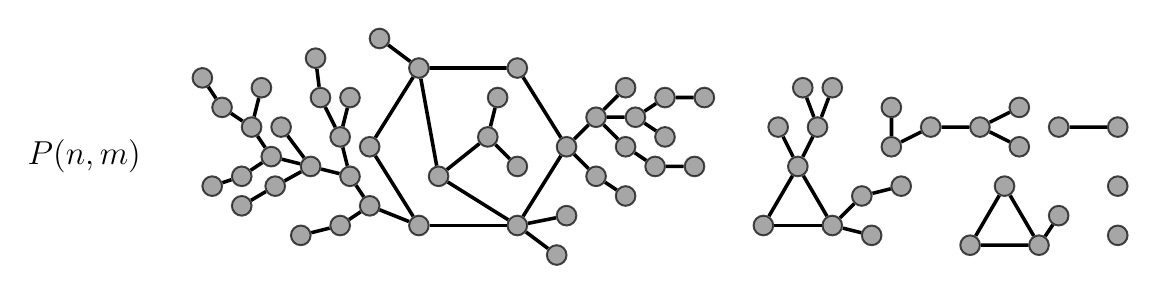
\begin{tikzpicture}[scale=1.25, line width=0.45mm, every node/.style={circle,fill=gray,draw,line width=0.25mm,inner sep=0,minimum size=0.25cm}]
		
		\node (A) at (0,0) [circle,draw, opacity=\op]  {};
		\node (B) at (1,0) [circle,draw, opacity=\op]  {};
		\node (C) at (1.5,0.8) [circle,draw, opacity=\op]  {};
		\node (D) at (1,1.6) [circle,draw, opacity=\op]  {};
		\node (E) at (0,1.6) [circle,draw, opacity=\op]  {};
		\node (F) at (-0.5,0.8) [circle,draw, opacity=\op]  {};
		\node (G) at (0.2,0.5) [circle,draw, opacity=\op]  {};
		\node (H) at (0.7,0.9) [circle,draw, opacity=\op]  {};
		\node (I) at (0.8,1.3) [circle,draw, opacity=\op]  {};
		\node (J) at (1,0.6) [circle,draw, opacity=\op]  {};
		\node (K) at (1.8,1.1) [circle,draw, opacity=\op]  {};
		\node (L) at (1.8,0.5) [circle,draw, opacity=\op]  {};
		\node (M) at (2.1,1.4) [circle,draw, opacity=\op]  {};
		\node (N) at (2.2,1.1) [circle,draw, opacity=\op]  {};
		\node (O) at (2.1,0.8) [circle,draw, opacity=\op]  {};
		\node (P) at (2.1,0.3) [circle,draw, opacity=\op]  {};
		\node (Q) at (2.5,1.3) [circle,draw, opacity=\op]  {};
		\node (R) at (2.5,0.9) [circle,draw, opacity=\op]  {};
		\node (S) at (2.4,0.6) [circle,draw, opacity=\op]  {};
		\node (T) at (2.9,1.3) [circle,draw, opacity=\op]  {};
		\node (U) at (2.8,0.6) [circle,draw, opacity=\op]  {};
		\node (V) at (1.5,0.1) [circle,draw, opacity=\op]  {};
		\node (W) at (1.4,-0.3) [circle,draw, opacity=\op]  {};
		\node (X) at (-0.4,1.9) [circle,draw, opacity=\op]  {};
		\node (Y) at (-0.5,0.2) [circle,draw, opacity=\op]  {};
		\node (Z) at (-0.7,0.5) [circle,draw, opacity=\op]  {};
		\node (AA) at (-0.8,0) [circle,draw, opacity=\op]  {};
		\node (AB) at (-0.8,0.9) [circle,draw, opacity=\op]  {};
		\node (AC) at (-1.1,0.6) [circle,draw, opacity=\op]  {};
		\node (AD) at (-1.2,-0.1) [circle,draw, opacity=\op]  {};
		\node (AE) at (-1.4,1) [circle,draw, opacity=\op]  {};	
		\node (AF) at (-1.5,0.7) [circle,draw, opacity=\op]  {};
		\node (AG) at (-1.46,0.4) [circle,draw, opacity=\op]  {};
		\node (AH) at (-0.7,1.3) [circle,draw, opacity=\op]  {};
		\node (AI) at (-1,1.3) [circle,draw, opacity=\op]  {};
		\node (AJ) at (-1.05,1.7) [circle,draw, opacity=\op]  {};
		\node (AK) at (-1.7,1) [circle,draw, opacity=\op]  {};
		\node (AL) at (-1.8,0.5) [circle,draw, opacity=\op]  {};
		\node (AM) at (-1.8,0.2) [circle,draw, opacity=\op]  {};	
		\node (AN) at (-1.6,1.4) [circle,draw, opacity=\op]  {};
		\node (AO) at (-2,1.2) [circle,draw, opacity=\op]  {};
		\node (AP) at (-2.1,0.4) [circle,draw, opacity=\op]  {};		
		\node (AQ) at (-2.2,1.5) [circle,draw, opacity=\op]  {};	
		
		\draw[-] (A) to (B);
		\draw[-] (B) to (C);
		\draw[-] (C) to (D);
		\draw[-] (D) to (E);
		\draw[-] (E) to (F);
		\draw[-] (F) to (A);
		\draw[-] (B) to (G);
		\draw[-] (E) to (G);
		\draw[-] (G) to (H);
		\draw[-] (H) to (I);
		\draw[-] (H) to (J);
		\draw[-] (C) to (K);
		\draw[-] (C) to (L);
		\draw[-] (K) to (M);
		\draw[-] (K) to (N);
		\draw[-] (K) to (O);
		\draw[-] (L) to (P);
		\draw[-] (N) to (Q);
		\draw[-] (N) to (R);
		\draw[-] (O) to (S);
		\draw[-] (Q) to (T);
		\draw[-] (S) to (U);
		\draw[-] (B) to (V);
		\draw[-] (B) to (W);
		\draw[-] (E) to (X);
		\draw[-] (A) to (Y);
		\draw[-] (Y) to (Z);
		\draw[-] (Y) to (AA);
		\draw[-] (Z) to (AB);
		\draw[-] (Z) to (AC);
		\draw[-] (AA) to (AD);
		\draw[-] (AC) to (AE);
		\draw[-] (AC) to (AF);
		\draw[-] (AC) to (AG);
		\draw[-] (AB) to (AH);
		\draw[-] (AB) to (AI);
		\draw[-] (AI) to (AJ);
		\draw[-] (AF) to (AK);
		\draw[-] (AF) to (AL);
		\draw[-] (AG) to (AM);
		\draw[-] (AK) to (AN);
		\draw[-] (AK) to (AO);
		\draw[-] (AL) to (AP);
		\draw[-] (AO) to (AQ);
		
		\node (AR) at (3.5,0) [circle,draw, opacity=\op]  {};
		\node (AS) at (4.2,0) [circle,draw, opacity=\op]  {};		
		\node (AT) at (3.85,0.6) [circle,draw, opacity=\op]  {};
		\node (AU) at (3.65,1) [circle,draw, opacity=\op]  {};
		\node (AV) at (4.05,1) [circle,draw, opacity=\op]  {};
		\node (AW) at (3.9,1.4) [circle,draw, opacity=\op]  {};
		\node (AX) at (4.2,1.4) [circle,draw, opacity=\op]  {};
		\node (AY) at (4.5,0.3) [circle,draw, opacity=\op]  {};
		\node (AZ) at (4.6,-0.1) [circle,draw, opacity=\op]  {};
		\node (BA) at (4.9,0.4) [circle,draw, opacity=\op]  {};
		
		\draw[-] (AR) to (AS);
		\draw[-] (AS) to (AT);
		\draw[-] (AT) to (AR);
		\draw[-] (AT) to (AU);
		\draw[-] (AT) to (AV);
		\draw[-] (AV) to (AW);
		\draw[-] (AV) to (AX);
		\draw[-] (AS) to (AY);
		\draw[-] (AS) to (AZ);
		\draw[-] (AY) to (BA);
		
		\node (BB) at (4.8,1.2) [circle,draw, opacity=\op]  {};
		\node (BC) at (4.8,0.8) [circle,draw, opacity=\op]  {};		
		\node (BD) at (5.2,1) [circle,draw, opacity=\op]  {};
		\node (BE) at (5.7,1) [circle,draw, opacity=\op]  {};
		\node (BF) at (6.1,1.2) [circle,draw, opacity=\op]  {};
		\node (BG) at (6.1,0.8) [circle,draw, opacity=\op]  {};
		
		\draw[-] (BB) to (BC);
		\draw[-] (BC) to (BD);
		\draw[-] (BD) to (BE);
		\draw[-] (BE) to (BF);
		\draw[-] (BE) to (BG);
		
		\node (BH) at (5.6,-0.2) [circle,draw, opacity=\op]  {};
		\node (BI) at (6.3,-0.2) [circle,draw, opacity=\op]  {};		
		\node (BJ) at (5.95,0.4) [circle,draw, opacity=\op]  {};
		\node (BK) at (6.5,0.1) [circle,draw, opacity=\op]  {};
		
		\draw[-] (BH) to (BI);
		\draw[-] (BI) to (BJ);
		\draw[-] (BJ) to (BH);
		\draw[-] (BI) to (BK);
		
		\node (BL) at (6.5,1) [circle,draw, opacity=\op]  {};
		\node (BM) at (7.1,1) [circle,draw, opacity=\op]  {};
		
		\draw[-] (BL) to (BM);
		
		\node (BN) at (7.1,0.4) [circle,draw, opacity=\op]  {};
		\node (BO) at (7.1,-0.1) [circle,draw, opacity=\op]  {};
		
		\node () at (-3.4,0.7) [rectangle,draw=none,fill=none]  {\large $P(n,m)$};

	\end{tikzpicture}

\hdashrule{14.5cm}{1pt}{1.5mm}
\vspace{0.5cm}

	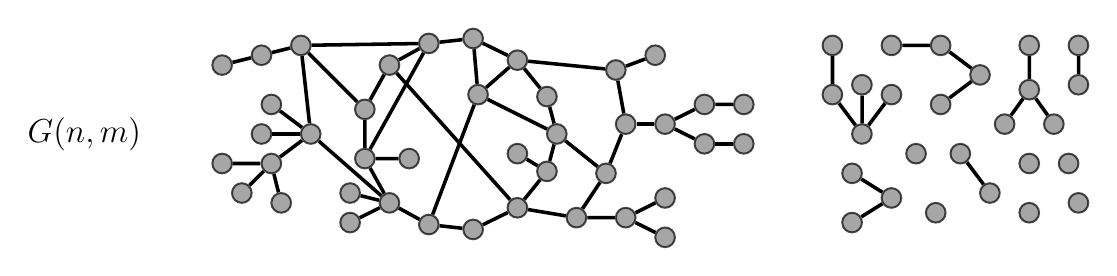
\begin{tikzpicture}[scale=1.25, line width=0.45mm, every node/.style={circle,fill=gray,draw,line width=0.25mm,inner sep=0,minimum size=0.25cm}]
		\node (A) at (1,0) [circle,draw, opacity=\op]  {};
		\node (B) at (0.9,0.38) [circle,draw, opacity=\op]  {};
		\node (C) at (0.6,0.75) [circle,draw, opacity=\op]  {};
		\node (D) at (0.15,0.97) [circle,draw, opacity=\op]  {};
		\node (E) at (-0.3,0.92) [circle,draw, opacity=\op]  {};
		\node (F) at (-0.7,0.7) [circle,draw, opacity=\op]  {};
		\node (G) at (-0.95,0.25) [circle,draw, opacity=\op]  {};
		\node (H) at (-0.95,-0.25) [circle,draw, opacity=\op]  {};
		\node (I) at (-0.7,-0.7) [circle,draw, opacity=\op]  {};
		\node (J) at (-0.3,-0.92) [circle,draw, opacity=\op]  {};
		\node (K) at (0.15,-0.97) [circle,draw, opacity=\op]  {};
		\node (L) at (0.6,-0.75) [circle,draw, opacity=\op]  {};
		\node (M) at (0.9,-0.38) [circle,draw, opacity=\op]  {};
		\node (N) at (0.2,0.4) [circle,draw, opacity=\op]  {};
		\node (O) at (-1.5,0) [circle,draw, opacity=\op]  {};
		\node (P) at (-1.6,0.9) [circle,draw, opacity=\op]  {};
		\node (Q) at (1.2,-0.85) [circle,draw, opacity=\op]  {};
		\node (R) at (1.5,-0.4) [circle,draw, opacity=\op]  {};
		\node (S) at (1.7,0.1) [circle,draw, opacity=\op]  {};
		\node (T) at (1.6,0.65) [circle,draw, opacity=\op]  {};
		\node (U) at (2.1,0.1) [circle,draw, opacity=\op]  {};
		\node (V) at (2.5,0.3) [circle,draw, opacity=\op]  {};
		\node (W) at (2.5,-0.1) [circle,draw, opacity=\op]  {};
		\node (X) at (2.9,0.3) [circle,draw, opacity=\op]  {};
		\node (Y) at (2.9,-0.1) [circle,draw, opacity=\op]  {};
		\node (Z) at (-2.2,-0.6) [circle,draw, opacity=\op]  {};
		\node (AA) at (-1.8,-0.7) [circle,draw, opacity=\op]  {};
		\node (AB) at (-1.9,0.3) [circle,draw, opacity=\op]  {};
		\node (AC) at (-2,0) [circle,draw, opacity=\op]  {};
		\node (AD) at (-1.9,-0.3) [circle,draw, opacity=\op]  {};
		\node (AE) at (-2.4,-0.3) [circle,draw, opacity=\op]  {};
		\node (AF) at (1.7,-0.85) [circle,draw, opacity=\op]  {};
		\node (AG) at (2.1,-0.65) [circle,draw, opacity=\op]  {};
		\node (AH) at (2.1,-1.05) [circle,draw, opacity=\op]  {};
		\node (AI) at (-1.1,-0.6) [circle,draw, opacity=\op]  {};
		\node (AJ) at (-1.1,-0.9) [circle,draw, opacity=\op]  {};
		\node (AK) at (-2,0.8) [circle,draw, opacity=\op]  {};
		\node (AL) at (-2.4,0.7) [circle,draw, opacity=\op]  {};
		\node (AM) at (0.6,-0.2) [circle,draw, opacity=\op]  {};
		\node (AN) at (2,0.8) [circle,draw, opacity=\op]  {};
		\node (AO) at (-0.5,-0.25) [circle,draw, opacity=\op]  {};
		
		\draw[-] (A) to (B);
		\draw[-] (B) to (C);
		\draw[-] (C) to (D);
		\draw[-] (D) to (E);
		\draw[-] (E) to (F);
		\draw[-] (F) to (G);
		\draw[-] (G) to (H);
		\draw[-] (H) to (I);
		\draw[-] (I) to (J);
		\draw[-] (J) to (K);
		\draw[-] (K) to (L);
		\draw[-] (L) to (M);
		\draw[-] (M) to (A);
		\draw[-] (A) to (N);
		\draw[-] (C) to (N);
		\draw[-] (D) to (N);
		\draw[-] (J) to (N);
		\draw[-] (F) to (L);
		\draw[-] (E) to (H);
		\draw[-] (I) to (O);
		\draw[-] (E) to (P);
		\draw[-] (G) to (P);
		\draw[-] (O) to (P);
		\draw[-] (L) to (Q);
		\draw[-] (Q) to (R);
		\draw[-] (R) to (S);
		\draw[-] (S) to (T);
		\draw[-] (C) to (T);
		\draw[-] (A) to (R);
		\draw[-] (S) to (U);
		\draw[-] (U) to (V);
		\draw[-] (U) to (W);
		\draw[-] (V) to (X);
		\draw[-] (W) to (Y);
		\draw[-] (AD) to (Z);
		\draw[-] (AD) to (AA);
		\draw[-] (O) to (AB);
		\draw[-] (O) to (AC);
		\draw[-] (O) to (AD);
		\draw[-] (AD) to (AE);
		\draw[-] (Q) to (AF);
		\draw[-] (AF) to (AG);
		\draw[-] (AF) to (AH);
		\draw[-] (I) to (AI);
		\draw[-] (I) to (AJ);
		\draw[-] (P) to (AK);
		\draw[-] (AK) to (AL);
		\draw[-] (M) to (AM);
		\draw[-] (T) to (AN);
		\draw[-] (H) to (AO);
		
		\node (AP) at (4.1,0) [circle,draw, opacity=\op]  {};
		\node (AQ) at (3.8,0.4) [circle,draw, opacity=\op]  {};
		\node (AR) at (4.1,0.5) [circle,draw, opacity=\op]  {};
		\node (AS) at (4.4,0.4) [circle,draw, opacity=\op]  {};
		\node (AT) at (3.8,0.9) [circle,draw, opacity=\op]  {};
		
		\draw[-] (AP) to (AQ);	
		\draw[-] (AP) to (AR);
		\draw[-] (AP) to (AS);
		\draw[-] (AQ) to (AT);
		
		\node (AU) at (4.4,0.9) [circle,draw, opacity=\op]  {};
		\node (AV) at (4.9,0.9) [circle,draw, opacity=\op]  {};
		\node (AW) at (5.3,0.6) [circle,draw, opacity=\op]  {};
		\node (AX) at (4.9,0.3) [circle,draw, opacity=\op]  {};
		
		\draw[-] (AU) to (AV);
		\draw[-] (AV) to (AW);
		\draw[-] (AW) to (AX);
		
		\node (AY) at (4,-0.4) [circle,draw, opacity=\op]  {};
		\node (AZ) at (4,-0.9) [circle,draw, opacity=\op]  {};
		\node (BA) at (4.4,-0.65) [circle,draw, opacity=\op]  {};
		
		\draw[-] (AY) to (BA);
		\draw[-] (AZ) to (BA);
		
		\node (BB) at (5.8,0.9) [circle,draw, opacity=\op]  {};
		\node (BC) at (5.8,0.45) [circle,draw, opacity=\op]  {};
		\node (BD) at (5.55,0.1) [circle,draw, opacity=\op]  {};
		\node (BE) at (6.05,0.1) [circle,draw, opacity=\op]  {};
		
		\draw[-] (BB) to (BC);
		\draw[-] (BC) to (BD);
		\draw[-] (BC) to (BE);
		
		\node (BF) at (5.1,-0.2) [circle,draw, opacity=\op]  {};
		\node (BG) at (5.4,-0.6) [circle,draw, opacity=\op]  {};
		
		\draw[-] (BF) to (BG);
		
		\node (BH) at (6.3,0.9) [circle,draw, opacity=\op]  {};
		\node (BI) at (6.3,0.5) [circle,draw, opacity=\op]  {};
		
		\draw[-] (BH) to (BI);
		
		\node (BJ) at (4.85,-0.8) [circle,draw, opacity=\op]  {};
		\node (BK) at (5.8,-0.3) [circle,draw, opacity=\op]  {};
		\node (BL) at (6.2,-0.3) [circle,draw, opacity=\op]  {};
		\node (BM) at (6.3,-0.7) [circle,draw, opacity=\op]  {};
		\node (BN) at (5.8,-0.8) [circle,draw, opacity=\op]  {};
		\node (BO) at (4.65,-0.2) [circle,draw, opacity=\op]  {};
		
		\node () at (-3.8,0) [rectangle,draw=none,fill=none]  {\large $G(n,m)$};
		
	\end{tikzpicture}
	\caption{The typical structure of $P(n,m)$ in the regime $m=dn/2$ for $d\in (1,2)$ compared with $G(n,m)$: The edges are spread more evenly in $P(n,m)$ and as a consequence, the largest component of $P(n,m)$ is much \lq sparser\rq\ than in $G(n,m)$.}
	\label{fig:pnm-vs-gnm}
\end{figure}

\section{Main results}\label{sec:main_results}
In this section we summarise the main results of the thesis about the cycle and block structure, the number of cut vertices, the maximum degree, and the local structure of the random planar graph $P(n,m)$, as well as the number of accepted edges and the order of the largest component in the random planar graph process.

In \Cref{cha:cut_vertices,cha:cycles_blocks,cha:process,cha:max_degree,cha:local_structure} we prove that the results presented in this section hold for a much more general class of graphs, including series-parallel graphs, planar graphs, and graphs on a surface (see also \Cref{sub:other_classes}). However, for the sake of simplicity, we restrict our considerations in this section to $P(n,m)$ and the random planar graph process. In \Cref{subsec:results_cycles,subsec:results_maxdegree,subsec:results_local} we present our results on $P(n,m)$, compare them with known results on $G(n,m)$, and discuss similarities and differences of these two models. Finally, in \Cref{subsec:results_process} we state our results on the random planar graph process.

As discussed in \Cref{sec:planar_vs_erdoes}, all asymptotic results on $G(n,m)$ can be transferred to $P(n,m)$ as long as $m\leq n/2+\bigo{n^{2/3}}$. Therefore, we focus on the case $m=n/2+s$ for $s^3n^{-2}\to \infty$. Especially interesting is the so-called {\em weakly supercritical regime} when $s=\smallo{n}$, because it is the \lq first\rq\ regime in which there might be significant differences between $P(n,m)$ and $G(n,m)$. Throughout the thesis we have different upper bounds on $s$. The weakly supercritical regime is included in all cases and in most results we even cover \lq almost\rq\ the whole sparse regime where $s\leq n/2+\smallo{n}$.

To provide a finer insight in the structure of $P(n,m)$, we state our results not only for the whole random planar graph $P=P(n,m)$, but also for its largest component $L=L(P)$ and its remaining part $R=R(P)=P\setminus L$. 

Given a graph $H$, we denote by $\vertexSet{H}$ the vertex set of $H$ and by $\edgeSet{H}$ its edge set. Furthermore, we let $\numberVertices{H}:=\left|\vertexSet{H}\right|$ be the order of $H$, i.e., the number of vertices in $H$, and $\numberEdges{H}:=\left|\edgeSet{H}\right|$ the number of edges. We refer to \Cref{CBsub:asymptotic_notation} for details on the asymptotic notation we use in our statements.

\subsection{Cycles, blocks, and cut vertices}\label{subsec:results_cycles}
In this subsection we present results on the length of the longest and shortest cycles, the order of the largest block, and the number of blocks and cut vertices in the random planar graph $P(n,m)$. Given a graph $H$, we denote by $c(H)$ the circumference of $H$, i.e., the length of the longest cycle in $H$, and by $g(H)$ the girth of $H$, i.e., the length of the shortest cycle in $H$.

\begin{thm}\label{thm:main_cycle}
Let $m=m(n)=n/2+s$ for $s^3n^{-2}\to\infty$ and $s=\smallo{n}$. Furthermore, let $P=P(n,m)$ be the random planar graph, $L=L(P)$ its largest component, and $R=R(P)$ its remaining part. Then whp the longest cycle in $P(n,m)$ is contained in the largest component $L$. Moreover, the circumference $c(L)$ of the largest component, the girth $g(L)$ of the largest component, and the circumference $c(R)$ of the remaining part in $P(n,m)$ satisfy the following. 
\begin{enumerate}
    \item 
    $c(L)=\OmegaP{n^{1/3}\log\left(sn^{-2/3}\right)}$, whp $c(L)=\bigo{sn^{-1/3}}$;
    \item
    $g(L)=\ThetaP{ns^{-1}}$;
    \item
    $c(R)=\ThetaP{n^{1/3}}$.
\end{enumerate}
\end{thm}
In \Cref{cha:cycles_blocks} we restate \Cref{thm:main_cycle} in a more general setting (see \Cref{CBthm:main1,CBthm:general}). In the following table we compare \Cref{thm:main_cycle} with corresponding results on $G(n,m)$ due to \Luczak\ \cite{Luczak1991b}.


\begin{center}
\def\arraystretch{1.8}\tabcolsep=10pt
\begin{tabular}{l|c|c|c}
    & $c(L)$ & $g(L)$ & $c(R)$ \\[0.1cm]
    \hline
    $P(n,m)$ & $\OmegaP{n^{1/3}\log\left(sn^{-2/3}\right)}$, $\bigo{sn^{-1/3}}$& $\ThetaP{ns^{-1}}$ & $\ThetaP{n^{1/3}}$ \\[0.1cm]
    \hline
    $G(n,m)$ & $\Th{s^2n^{-1}}$ & $\ThetaP{ns^{-1}}$ & $\ThetaP{ns^{-1}}$
\end{tabular}
\end{center}
We emphasise that in both models whp the longest cycle is contained in the largest component. However, in $P(n,m)$ it is much shorter than in $G(n,m)$, because $sn^{-1/3}=\smallo{s^2n^{-1}}$. In contrast, the longest cycle in the remaining part is significantly longer in $P(n,m)$, since $n^{1/3}=\smallomega{ns^{-1}}$. This is in perfect accordance with the intuitions in \Cref{sec:planar_vs_erdoes} that the largest component of $P(n,m)$ is much sparser than in $G(n,m)$, while the remaining part is much denser. In view of this heuristic, $P(n,m)$ should have much less cycles than $G(n,m)$, and therefore, one would perhaps expect that the girth of the largest component $g(L)$ should be larger in $P(n,m)$ than in $G(n,m)$. However, \Cref{thm:main_cycle} reveals that this is not the case and $g(L)$ is of the same order in the two models. Thus, it seems that the restriction of planarity in $P(n,m)$ has a larger impact on long cycles than on short ones.

Another well-studied structure related to cycles are blocks, i.e., maximal 2-connected subgraphs. The next result (which is just a reformulation of \Cref{CBthm:block_structure}) provides the order of the $i$-th largest block in $P(n,m)$ and the number of blocks in the largest component of $P(n,m)$.
\begin{thm}\label{thm:main_block}
Let $P=P(n,m)$ be the random planar graph and $m=m(n)=n/2+s$ for $s^3n^{-2}\to\infty$ and $s=\smallo{n}$. Then the order of the largest block in $P$ is $\ThetaP{sn^{-1/3}}$ and for $i\geq 2$, the order of the $i$-th largest block is $\ThetaP{s^{2/3}n^{-1/9}}$. Furthermore, whp the number of blocks in the largest component of $P$ is $\Th{sn^{-2/3}}$.
\end{thm}
In the following table we summarise the results in \Cref{thm:main_block} to compare them with corresponding results on $G(n,m)$ due to \Luczak\ \cite{Luczak1991b}. We observe amongst others that the largest block in $P(n,m)$ is much smaller than in $G(n,m)$, while the second largest block and the number of blocks in the largest component are much larger.

\begin{center}
\def\arraystretch{1.8}\tabcolsep=10pt
\begin{tabular}{l|c|c|c}
    & order largest block & order $i$-th largest block, $i\geq 2$ & $\# \text{blocks in } L$ \\[0.1cm]
    \hline
    $P(n,m)$ & $\ThetaP{sn^{-1/3}}$ & $\ThetaP{s^{2/3}n^{-1/9}}$ & $\Th{sn^{-2/3}}$ \\[0.1cm]
    \hline
    $G(n,m)$ & $\Th{s^2n^{-1}}$ & $\OP{ns^{-1}}$ & $\OP{1}$
\end{tabular}
\end{center}

A vertex in a graph is called a {\em cut vertex} if removing it and all its incident edges increases the number of components. Given a graph $H$, we denote by $\cv{H}$ the fraction of cut vertices in $H$, that is, the number of cut vertices in $H$ divided by the total number of vertices in $H$. The next result (a restatement of \Cref{thm:planar_sup}) provides the fraction of cut vertices in $P(n,m)$, its largest component, and its remaining part. 
\begin{thm}\label{thm:main_cut_vertices}
Let $m=m(n)=n/2+s$ be such that $s^3n^{-2}\to \infty$, $s\leq n/2+\smallo{n\left(\log n\right)^{-2/3}}$, and $2m/n\to d\in [1,2]$. Furthermore, let $P=P(n,m)$ be the random planar graph, $L=L(P)$ its largest component, and $R=R(P)$ its remaining part. Then whp $\cv{L}=1-e^{-1}+\smallo{1}$, $\cv{R}=1-2e^{-1}+\smallo{1}$, and $\cv{P}=1-(3-d)e^{-1}+\smallo{1}$.
\end{thm}

We note that the assumption $s\leq n/2+\smallo{n\left(\log n\right)^{-2/3}}$ is \lq inherited\rq\ from a result in \cite{KangMosshammerSpruessel2020}, which we apply in our proofs. For comparison, we also provide results on the number of cut vertices in $G(n,m)$. To that end, we denote by $\beta_d$ the unique positive solution of the equation 
\begin{align}\label{eq:7}
1-x=e^{-dx} \quad \text{for } d>1
\end{align}
and we let $\beta_d:=0$ for $d=1$. We observe that $\beta_d$ is the survival probability of a \GW\ process with Poisson offspring distribution with mean $d$. If $m=m(n)=n/2+s$ is such that $s^3n^{-2}\to \infty$, $s\leq n/2+\smallo{n\left(\log n\right)^{-2/3}}$, and $2m/n\to d\in [1,2]$, then whp the fraction $\cv{L}$ of cut vertices in the largest component, the fraction $\cv{R}$ of cut vertices in the remaining part, and the fraction $\Cv$ of cut vertices in the whole graph satisfy the following.

\begin{center}
   \def\arraystretch{1.8}\tabcolsep=3pt
\begin{tabular}{l|c|c|c}
    & $\cv{L}$ & $\cv{R}$ & $\Cv$ \\[0.1cm]
    \hline
    $P(n,m)$ & $1-e^{-1}+\smallo{1}$ & $1-2e^{-1}+\smallo{1}$ & $1-(3-d)e^{-1}+\smallo{1}$ \\[0.1cm]
    \hline
    $G(n,m)$ & $1\hspace{-0.035cm}-\hspace{-0.035cm}e^{-d\left(1-\beta_d\right)}\hspace{-0.035cm}+\hspace{-0.035cm}\smallo{1}$ & $1\hspace{-0.035cm}-\hspace{-0.035cm}\left(d+e^{d\beta_d}\right)e^{-d}\hspace{-0.035cm}+\hspace{-0.035cm}\smallo{1}$ & $1\hspace{-0.035cm}-\hspace{-0.035cm}\left(d+e^{d\beta_d}-d\beta_d\right)e^{-d}\hspace{-0.035cm}+\hspace{-0.035cm}\smallo{1}$
\end{tabular}
\end{center}


\begin{figure}
\begin{center}
 	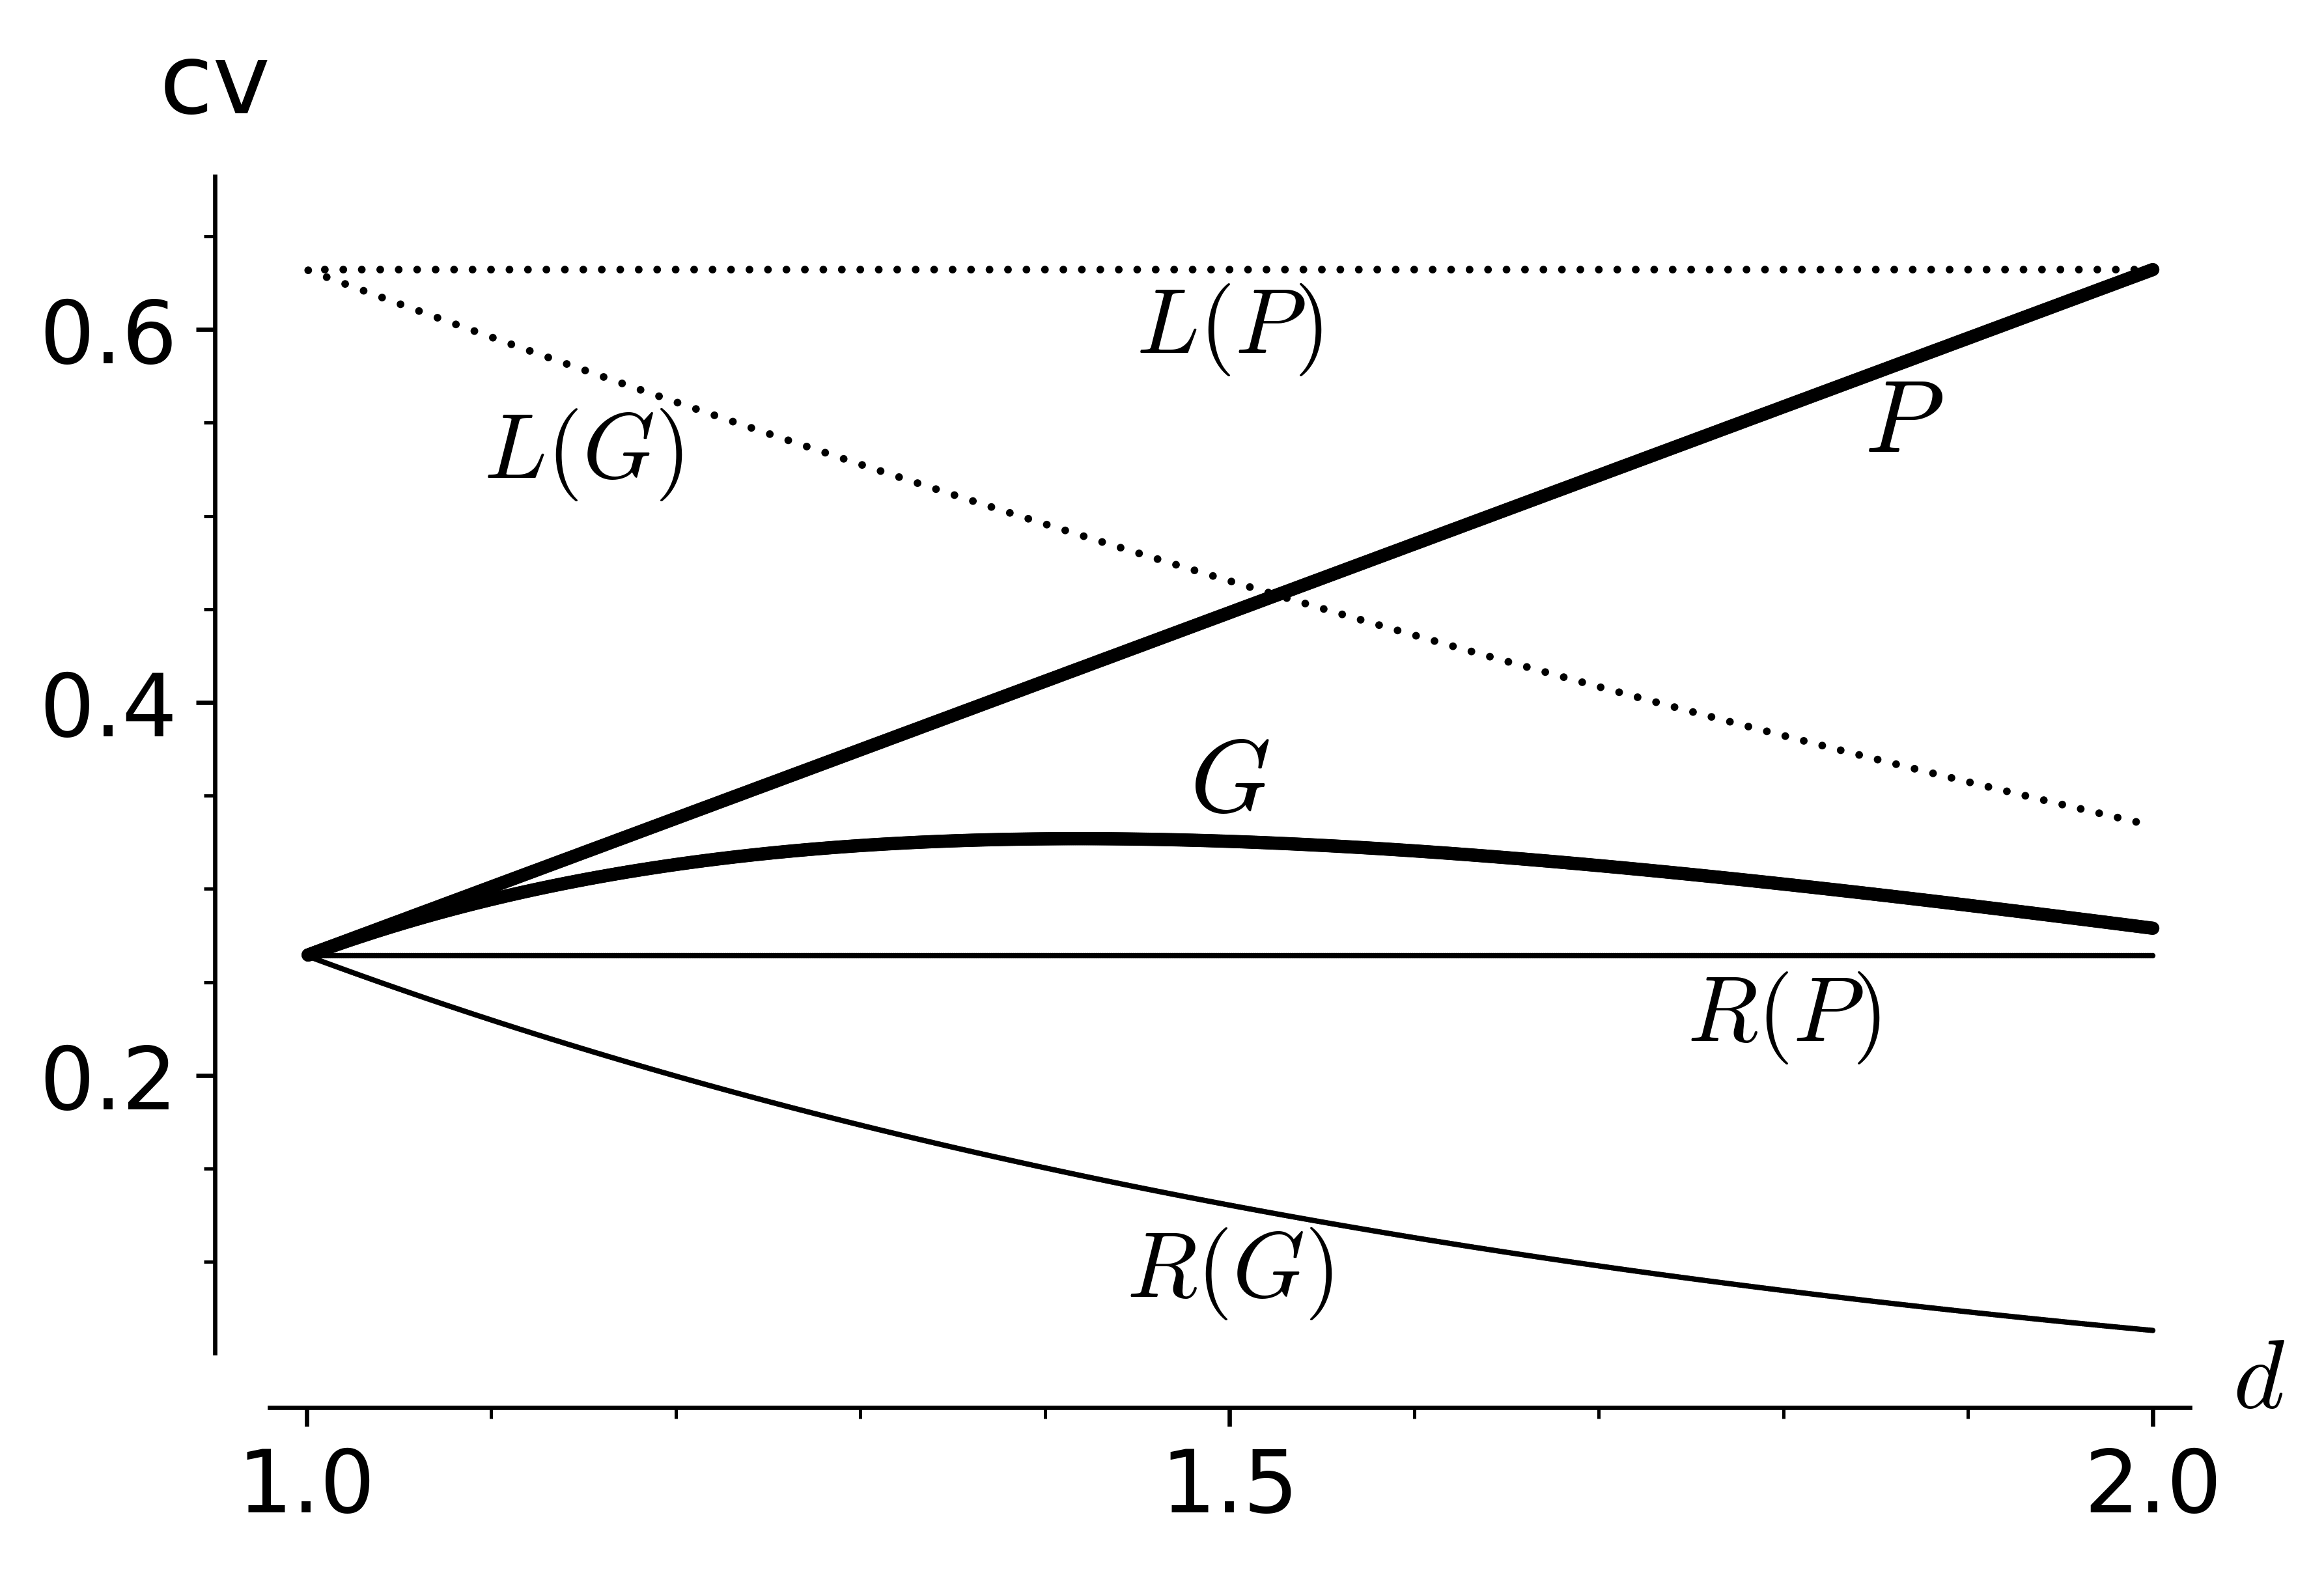
\includegraphics[scale=0.5]{cut-vertices.png}
 	\vspace{-0.5cm}
\end{center}
	\caption{Fraction of cut vertices in the random planar graph $P=P(n,m)$ and the \ER\ random graph $G=G(n,m)$, where $m=m(n)$ is such that $2m/n\to d\in [1,2]$.}
	\label{fig:cut_vertices}
\end{figure}

We refer to \Cref{fig:cut_vertices} for an illustration of the above results. Using \Cref{thm:average_degree} we can interpret them as follows: The largest component of $P(n,m)$ is much \lq sparser\rq\ than in $G(n,m)$ and therefore, it should be much more likely that the largest component gets disconnected when removing a random vertex from it. As a consequence, $\cv{L}$ is larger in $P(n,m)$ than in $G(n,m)$. To provide an insight into the behaviour of $\cv{R}$, we observe that a cut vertex has degree at least two. Furthermore, the remaining parts are typically quite sparse and therefore, we expect that most of the vertices with degree at least two are indeed cut vertices. Hence, the larger average degree in the remaining part of $P(n,m)$ leads also to a bigger number of cut vertices than in the remaining part of $G(n,m)$. As a consequence of these behaviours of $\cv{L}$ and $\cv{R}$, the random planar graph $P(n,m)$ contains typically more cut vertices than $G(n,m)$.

\subsection{Maximum degree}\label{subsec:results_maxdegree}

We denote by $\maxdegree{H}$ the maximum degree of a graph $H$. In this subsection we establish that there are only two values which are typically attained by the maximum degree $\maxdegree{P(n,m)}$ if the number of edges $m$ is \lq small\rq. However, if $m$ gets \lq larger\rq, the maximum degree is not concentrated on any subset of $[n]$ with bounded size. For comparison, we start with a concentration result on $\maxdegree{G(n,m)}$ by \Bollobas \cite{Bollobas1982}.

\begin{thm}[\hspace{1sp}\cite{Bollobas1982}]\label{thm:main_max_degree_gnm}
Let $m=m(n)=\smallo{n\log n}$. Then there exists a $D=D(n)$ such that whp $\maxdegree{G(n,m)}\in\left\{D,D+1\right\}$.
\end{thm}

\Cref{thm:main_max_degree_gnm} immediately implies that whp $\maxdegree{P(n,m)}$ takes one of two values if $m\leq n/2+\bigo{n^{2/3}}$. The next theorem says that this is still true as long as the average degree is at most two. Furthermore, also the maximum degrees of the largest component and the remaining part in $P(n,m)$ are concentrated at two values.

\begin{thm}\label{thm:main_max_degree_pnm}
Let $P=P(n,m)$, $L$ be the largest component of $P$, and $R=P\setminus L$ the remaining part of $P$. Assume that $m=m(n)=n/2+s$, where $s^3n^{-2}\to \infty$ and $s\leq n/2+n^{1-\delta}$ for some $\delta>0$. Then there exist $D_L=D_L(n)$, $D_R=D_R(n)$, and $D=D(n)=\left(1+\smallo{1}\right)\log n/\log\log n$ such that whp 
\begin{enumerate}
    \item 
    $\maxdegree{L}\in \left\{D_L, D_L+1\right\}$;
    \item
    $\maxdegree{R}\in \left\{D_R, D_R+1\right\}$;
    \item
    $\maxdegree{P}\in \left\{D, D+1\right\}$.
\end{enumerate}
\end{thm}

In \Cref{cha:max_degree} we prove a stronger version of \Cref{thm:main_max_degree_pnm}, which implies that for \lq many\rq\ $n\in\N$ the maximum degree $\maxdegree{P(n,m)}$ is even concentrated on a single value (see \Cref{MDthm:main}). \Cref{thm:main_max_degree_pnm} reveals that whp $\maxdegree{P(n,m)}=\smallomega{1}$, but nevertheless it typically attains only two values. As stated in \Cref{thm:main_max_degree_pnm}, the function $D$ may depend on the number of edges $m$. Somewhat surprising, the next result shows that we can find even a \lq uniform\rq\ $D$ that holds for {\em all} $m$ for which the average degree $2m/n$ tends to a constant in $(1,2)$. Moreover, whp the maximum degrees in the largest component and the remaining part differ at most by two.


\begin{thm}\label{thm:main_max_degree_independent}
Let $P=P(n,m)$, $L$ be the largest component of $P$, and $R=P\setminus L$ the remaining part of $P$. There exists a $D=D(n)\in \N$ such that for all $m=m(n)$ where $2m/n$ tends to a constant in $(1,2)$, we have whp
\begin{enumerate}
\item
$\maxdegree{L}\in \left\{D, D+1\right\}$;
\item
$\maxdegree{R}\in \left\{D-1, D\right\}$;
\item
$\maxdegree{P}\in \left\{D, D+1\right\}$.
\end{enumerate}
In particular, whp $\maxdegree{R}\leq\maxdegree{L}\leq\maxdegree{R}+2$.
\end{thm}

We note that although $P(n,0.99n)$ has almost twice as many edges as $P(n,0.51n)$, their maximum degrees typically differ at most by one. In contrast, $G(n,m)$ exhibits the following perhaps more \lq intuitive\rq\ behaviour (see \Cref{MDpro:ER} for details): If the average degree $2m/n$ grows, then both $\maxdegree{G(n,m)}$ and $\maxdegree{L}$ increase, while $\maxdegree{R}$ decreases. Furthermore, $\maxdegree{L}$ is significantly larger than $\maxdegree{R}$. Informally, we can interpret this striking difference between $P(n,m)$ and $G(n,m)$ as follows: If we increase the number of edges in $G(n,m)$, i.e., we add additional edges, then quite likely some of these edges are incident with vertices of \lq large\rq\ degree and therefore, the maximum degree $\maxdegree{G(n,m)}$ grows. On the other hand, if the number of edges in $P(n,m)$ is increased, then the edges are spread more and more evenly over the vertices such that the maximum degree $\maxdegree{P(n,m)}$ does not change.

We conclude this subsection by showing that the two-point concentration result on $\maxdegree{P(n,m)}$ cannot be extended to the \lq dense\rq\ regime where the average degree is larger than two. In this regime $\maxdegree{P(n,m)}$ is not concentrated on any subset of $[n]$ with bounded size. Before stating this result (a restatement of \Cref{MDthm:main_dense}), we mention a comparable statement in $G(n,m)$, which is due to \Bollobas \cite{Bollobas1982}.

\begin{thm}[\hspace{1sp}\cite{Bollobas1982}]
Let $m=m(n)=\smallomega{n\log n}$ and $m=\smallo{n^2}$. If $I=I(n)\subseteq[n]$ is such that whp $\maxdegree{G(n,m)}\in I$, then $|I|=\smallomega{1}$.
\end{thm}

\begin{thm}\label{thm:non_concentration}
Let $m=m(n)=\rounddown{dn/2}$ for a constant $d \in (2,6)$. If $I=I(n)\subseteq[n]$ is such that whp $\maxdegree{P(n,m)}\in I$, then $|I|=\smallomega{1}$. 
\end{thm}

We note that a planar graph on $n$ vertices has at most $3n-6$ edges, while a graph (without any constraint) can have up to $\binom{n}{2}$ many edges. Hence, it seems natural that the \lq threshold\rq\ for the two-point concentration of the maximum degree occurs much earlier in $P(n,m)$ than in $G(n,m)$, namely at $m\sim n$ instead of $m\sim n \log n$.

\subsection{Local weak limit}\label{subsec:results_local}
In this subsection we describe how $P(n,m)$ looks \lq locally\rq\ around a randomly chosen vertex. To state our main results, we introduce some notions, based on the concept of {\em local weak convergence} of random rooted graphs introduced by Benjamini and Schramm \cite{BenjaminiSchramm2001} and Aldous and Steele \cite{AldousSteele2004}: A {\em rooted graph} is a pair $\rootedGraph{H}{r}$ of a graph $H$ together with a vertex $r$ of $H$, which is called the root. For a rooted graph $(H,r)$ and $\ell\in\N$ we let $\ball{\ell}{H}{r}$ be the ball of radius $\ell$ and centre $r$ in $H$, which is the subgraph of $H$ induced on the vertices which have distance at most $\ell$ to $r$. Furthermore, we say that two rooted graphs $\rootedGraph{H_1}{r_1}$ and $\rootedGraph{H_2}{r_2}$ are {\em isomorphic} and write $\rootedGraph{H_1}{r_1}\cong\rootedGraph{H_2}{r_2}$ if there is an isomorphism of $H_1$ onto $H_2$ which maps $r_1$ to $r_2$. A {\em random} rooted graph is a random variable which takes rooted graphs as values. Given a sequence $\rootedGraph{G}{r}=\rootedGraph{G}{r}(n)$ of random rooted graphs, we say that another random rooted graph $\rootedGraph{G_0}{r_0}$ is the {\em local weak limit}, or for short the local limit, of $\rootedGraph{G}{r}$ if for all rooted graphs $\rootedGraph{H}{r_H}$ and $\ell\in\N$ we have
\begin{align*}
    \prob{\ball{\ell}{G}{r}\cong \rootedGraph{H}{r_H}}~~~\to~~~\prob{\ball{\ell}{G_0}{r_0}\cong \rootedGraph{H}{r_H}} \quad\quad \text{as } n\to \infty.
\end{align*}
In this case we write $\distributionalLimit{\rootedGraph{G}{r}}{\rootedGraph{G_0}{r_0}}$. We note that the local weak limit is also called distributional limit or Benjamini–Schramm
local weak limit.

We consider a random graph $G$ as a random rooted graph $\rootedGraph{G}{r}$ by first sampling the realisation $H$ of $G$ and then picking the root $r$ uniformly at random from the vertex set of $H$, which we denote by $r \ur \vertexSet{G}$. Roughly speaking, the local weak limit of $\rootedGraph{G}{r}$ \lq describes\rq\ the typical local structure of the random graph $G$.

We will see that the local weak limit of the random planar graph $P(n,m)$ is a \lq linear combination\rq\ of two random rooted graphs, which are themselves the local weak limits of two other well-known models of random graphs. The first one is the {\em \GW\ tree} with Poisson offspring distribution with mean $d$, denoted by $\gwt{d}$. It is well known that $\gwt{d}$ is the local weak limit of the \ER\ random graph $G(n,m)$ when $2m/n \to d$ (see e.g., \cite{DemboMontanari2010}).

\begin{thm}\label{thm:local_gnm}
Let $G=G(n,m)$, $m=m(n)$ be such that $2m/n\to d \in [0,\infty)$, and $r\ur\vertexSet{G}$. Then $\distributionalLimit{\rootedGraph{G}{r}}{\gwt{d}}$.
\end{thm}

The second random rooted graph which is related to the local weak limit of $P(n,m)$ is the so-called {\em Skeleton tree} $\skeletonTree$, which can be obtained by replacing independently each vertex of an infinite path (that starts at the root vertex of $\skeletonTree$) by a \GW\ tree $\gwt{1}$ (see \Cref{fig:skeleton_tree} for an illustration). Grimmett \cite{Grimmett198081} showed that the Skeleton tree $\skeletonTree$ is the local weak limit of the uniform random tree $T(n)$, which is a graph chosen uniformly at random from the set of all trees with vertex set $[n]$.

\begin{figure}[t]
\centering
	\begin{tikzpicture}[scale=1, line width=0.4mm, every node/.style={circle,fill=gray, inner sep=0, minimum size=0.22cm}]
		\node (1) at (0,0) [rectangle,draw]  {};
		\node (1a) at (0,-0.4) [draw=none, fill=none]  {$\root$};
		\node (2) at (1,0) [rectangle,draw]  {};
		\node (2a) at (1,-0.4) [draw=none, fill=none]  {$\root_2$};
		\node (3) at (2,0) [rectangle,draw]  {};
		\node (3a) at (2,-0.4) [draw=none, fill=none]  {$\root_3$};
		\node (4) at (3,0) [rectangle,draw]  {};
		\node (4a) at (3,-0.4) [draw=none, fill=none]  {$\root_4$};
		\node (5) at (4,0) [rectangle,draw]  {};
		\node (5a) at (4,-0.4) [draw=none, fill=none]  {$\root_5$};
		\node (6) at (5,0) [rectangle,draw]  {};
		\node (6a) at (5,-0.4) [draw=none, fill=none]  {$\root_6$};
		\node (7) at (6,0) [rectangle,draw]  {};
		\node (7a) at (6,-0.4) [draw=none, fill=none]  {$\root_7$};
		\node (8) at (7,0) [rectangle,draw]  {};
		\node (8a) at (7,-0.4) [draw=none, fill=none]  {$\root_8$};
		\draw[-] (1) to (2);
		\draw[-] (2) to (3);
		\draw[-] (3) to (4);
		\draw[-] (4) to (5);
		\draw[-] (5) to (6);
		\draw[-] (6) to (7);
		\draw[-] (7) to (8);
		\node (10) at (-0.3,0.7) [draw]  {};
		\node (11) at (0.3,0.7) [draw]  {};
		\draw[-] (1) to (10);
		\draw[-] (1) to (11);
		\node (12) at (-0.8,1.4) [draw]  {};
		\node (14) at (0.2,1.4) [draw]  {};
		\draw[-] (10) to (12);
		\draw[-] (10) to (14);
		\node (15) at (-0.8,2.1) [draw]  {};
		\node (16) at (-0.1,2.1) [draw]  {};
		\node (17) at (0.5,2.1) [draw]  {};
		\draw[-] (12) to (15);
		\draw[-] (14) to (16);
		\draw[-] (14) to (17);
		\node (18) at (-1.1,2.8) [draw]  {};
		\node (19) at (-0.5,2.8) [draw]  {};
		\node (13) at (0.5,2.8) [draw]  {};	
		\draw[-] (17) to (13);
		\draw[-] (15) to (18);
		\draw[-] (15) to (19);
		\node (20) at (-0.5,3.5) [draw]  {};
		\draw[-] (19) to (20);	
		\node (21) at (3.6,0.7) [draw]  {};
		\node (22) at (4,0.7) [draw]  {};
		\node (23) at (4.4,0.7) [draw]  {};
		\draw[-] (5) to (21);	
		\draw[-] (5) to (22);	
		\draw[-] (5) to (23);
		\node (24) at (3.3,1.4) [draw]  {};
		\node (25) at (3.9,1.4) [draw]  {};
		\node (26) at (4.4,1.4) [draw]  {};
		\draw[-] (21) to (24);	
		\draw[-] (21) to (25);	
		\draw[-] (23) to (26);
		\node (27) at (3.3,2.1) [draw]  {};
		\node (28) at (4,2.1) [draw]  {};
		\node (29) at (4.4,2.1) [draw]  {};
		\node (30) at (4.8,2.1) [draw]  {};
		\draw[-] (24) to (27);	
		\draw[-] (26) to (28);	
		\draw[-] (26) to (29);
		\draw[-] (26) to (30);	
		\node (31) at (3,2.8) [draw]  {};
		\node (32) at (3.6,2.8) [draw]  {};
		\node (33) at (4.4,2.8) [draw]  {};
		\draw[-] (27) to (31);	
		\draw[-] (27) to (32);	
		\draw[-] (29) to (33);
		\node (34) at (3.6,3.5) [draw]  {};
		\node (35) at (3,3.5) [draw]  {};
		\node (36) at (4.4,3.5) [draw]  {};
		\draw[-] (32) to (34);
		\draw[-] (31) to (35);	
		\draw[-] (33) to (36);	
		\node (38) at (3,4.2) [draw]  {};
		\node (39) at (4.15,4.2) [draw]  {};
		\node (37) at (4.65,4.2) [draw]  {};
		\draw[-] (36) to (37);	
		\draw[-] (35) to (38);	
		\draw[-] (36) to (39);	
		\node (40) at (7,0.7) [draw]  {};
		\node (41) at (6.6,1.4) [draw]  {};
		\node (42) at (7.4,1.4) [draw]  {};
		\node (42a) at (7,1.4) [draw]  {};
		\node (43) at (6.6,2.1) [draw]  {};	
		\draw[-] (8) to (40);	
		\draw[-] (40) to (41);	
		\draw[-] (40) to (42);
		\draw[-] (40) to (42a);
		\draw[-] (41) to (43);	
		\node (44) at (6,0.7) [draw]  {};
		\node (45) at (6,1.4) [draw]  {};	
		\draw[-] (7) to (44);	
		\draw[-] (44) to (45);	
		
		\node (48) at (1.75,0.7) [draw]  {};
		\node (49) at (2.25,0.7) [draw]  {};
		\draw[-] (3) to (48);
		\draw[-] (3) to (49);
		\node (46) at (7.8,0) [draw=none, fill=none]  {};
		\draw[->] (8) to (46);
		\node (47) at (8.2,1) [draw=none, fill=none]  {\Huge $\ldots$};
	\end{tikzpicture}
	\caption{The Skeleton tree $\skeletonTree$ with root $r$: The vertices $r, r_2, r_3, \ldots$ of an infinite path are the roots of independent \GW\ trees with Poisson offspring distribution with mean one.}
	\label{fig:skeleton_tree}
\end{figure}

\begin{thm}[\hspace{1sp}\cite{Grimmett198081}]
Let $T=T(n)$ be the uniform random tree and $r\ur\vertexSet{T}$. Then we have $\distributionalLimit{\rootedGraph{T}{r}}{\skeletonTree}$.
\end{thm}

To phrase the local weak limit of $P(n,m)$, we introduce the notion of a \lq linear combination\rq\ of two random rooted graphs: For a constant $a\in[0,1]$ and random rooted graphs $\rootedGraph{G_1}{r_1}$ and $\rootedGraph{G_2}{r_2}$, we denote by
\begin{align*}
a\rootedGraph{G_1}{r_1}+(1-a)\rootedGraph{G_2}{r_2}   
\end{align*}
the random rooted graph which can be obtained as follows: First we choose $i=1$ with probability $a$ and $i=2$ with probability $1-a$. Then we sample a realisation of $\rootedGraph{G_i}{r_i}$ to obtain $a\rootedGraph{G_1}{r_1}+(1-a)\rootedGraph{G_2}{r_2}$.

\begin{thm}\label{thm:main_local}
Let $P=P(n,m)$, $L=L(P)$ be the largest component of $P$, and $R=R(P)=P\setminus L$ the remaining part of $P$. Assume $m=m(n)=n/2+s$ where $s^3n^{-2}\to \infty$, $s\leq n/2+\smallo{n\left(\log n\right)^{-2/3}}$, and $2m/n\to d\in[1,2]$. Moreover, let $r_L\ur \vertexSet{L}$, $r_R\ur \vertexSet{R}$, and $r\ur \vertexSet{P}$. Then we have
\begin{enumerate}
    \item\label{thm:main_local_a}
    $\distributionalLimit{\rootedGraph{L}{r_L}}{\skeletonTree}$;
    \item\label{thm:main_local_b}
    $\distributionalLimit{\rootedGraph{R}{r_R}}{\gwt{1}}$;
    \item\label{thm:main_local_c}
    $\distributionalLimit{\rootedGraph{P}{r}}{(d-1)\skeletonTree+(2-d)\gwt{1}}$.
\end{enumerate}
\end{thm}

In \Cref{cha:local_structure} we state a more detailed version of \Cref{thm:main_local} (see \Cref{LSthm:main1,LSthm:main2,LSthm:main3}). In \Cref{thm:average_degree} we saw that the average degree of the largest component $L$ in $P(n,m)$ is around two and therefore, close to the average degree of a tree. \Cref{thm:main_local}\ref{thm:main_local_a} shows that locally $L$ is even \lq indistinguishable\rq\ from the uniform random tree. \Cref{thm:main_local}\ref{thm:main_local_b} implies that the remaining part $R$ of $P(n,m)$ has the same local limit as the \ER\ random graph with average degree one. Furthermore, \Cref{thm:main_local}\ref{thm:main_local_c} reveals a smooth transition from the case $d\sim 1$, where $P(n,m)$ looks locally like $G(n,m)$, to $d\sim 2$, where the local structure of $P(n,m)$ is close to that of $T(n)$.

To compare the local structures of $P(n,m)$ and $G(n,m)$, we consider the \lq local expansion\rq\ of rooted graphs. More formally, for a rooted graph $\rootedGraph{H}{r}$ and $\ell\in\N$, let $\expansion{\ell}{H}{r}$ be the number of vertices in $H$ whose distance to $r$ is exactly $\ell$. We note that $\expec{\expansionP{\ell}{\skeletonTree}}=\ell+1$ and $\expec{\expansionP{\ell}{\gwt{d}}}=d^\ell$. Together with \Cref{thm:local_gnm,thm:main_local} this indicates that for a vertex $r$ in $P(n,m)$ there are on average around $1+(d-1)\ell$ vertices with distance $\ell$ to $r$, while for a vertex in $G(n,m)$ there are $d^\ell$ such vertices. For $d>1$ this shows a big difference in the local structures of $P(n,m)$ and $G(n,m)$, which can be summarised as follows: Due to the restriction of planarity, $P(n,m)$ \lq expands\rq\ locally around a vertex only \lq linearly\rq, while $G(n,m)$ locally \lq expands exponentially\rq\ (see \Cref{fig:local} for an illustration).

\def\lw{1pt}
\begin{figure}[t]
\centering
\begin{tikzpicture}[line cap=round,line join=round,>=triangle 45,x=1cm,y=1cm,scale=0.55]
\draw [line width=0.8pt,dotted,opacity=0.3] (0,0) circle (1cm);
\draw [line width=0.8pt,dotted,opacity=0.3] (0,0) circle (2cm);
\draw [line width=0.8pt,dotted,opacity=0.3] (0,0) circle (3cm);
\draw [line width=0.8pt,dotted,opacity=0.3] (0,0) circle (4cm);
\draw [line width=0.8pt,dotted,opacity=0.3] (0,0) circle (5cm);


\draw [line width=\lw] (0,0)-- (1,0);
\draw [line width=\lw] (0,0)-- (-0.9661608270390681,-0.257940412295522);
\draw [line width=\lw] (0,0)-- (-0.7525766947068777,0.6585046078685182);
\draw [line width=\lw] (-0.7525766947068777,0.6585046078685182)-- (-1.8830411939684522,0.6739108708263027);
\draw [line width=\lw] (-0.7525766947068777,0.6585046078685182)-- (-0.32836792070015963,1.9728594751413628);
\draw [line width=\lw] (1,0)-- (2,0);
\draw [line width=\lw] (-1.8830411939684522,0.6739108708263027)-- (-2.984383742264281,0.3057019445614408);
\draw [line width=\lw] (-1.8830411939684522,0.6739108708263027)-- (-2.5988806275791636,1.4986058466433836);
\draw [line width=\lw] (2,0)-- (2.7248097893197807,1.255154019245086);
\draw [line width=\lw] (2,0)-- (3,0);
\draw [line width=\lw] (-2.5988806275791636,1.4986058466433836)-- (-3.530932225468438,1.879499300119184);
\draw [line width=\lw] (-2.984383742264281,0.3057019445614408)-- (-3.9857018995911777,0.3379058561127307);
\draw [line width=\lw] (2.7248097893197807,1.255154019245086)-- (3.0185444129259906,2.624574180165858);
\draw [line width=\lw] (3,0)-- (3.8606044921126097,-1.0467726379113746);
\draw [line width=\lw] (3,0)-- (4,0);
\draw [line width=\lw] (3.377161902244871,-2.143543208341228)-- (3,0);
\draw [line width=\lw] (4,0)-- (4.8488585514833655,1.2200699765614418);
\draw [line width=\lw] (4,0)-- (4.999994131644722,-0.007660516845794109);
\draw [line width=\lw] (3.8606044921126097,-1.0467726379113746)-- (4.523028944974421,-2.131245917984025);
\draw [line width=\lw] (3.0185444129259906,2.624574180165858)-- (3.787158929116345,3.264571525577949);
\draw [line width=\lw] (3.0185444129259906,2.624574180165858)-- (3.267705966674088,3.78445474478987);
\draw [line width=\lw] (-0.7525766947068777,0.6585046078685182)-- (-1.2766818089833283,1.5395075701701038);
\draw [line width=\lw] (2.7248097893197807,1.255154019245086)-- (3.5548501217650887,1.8338594852896262);
\draw [line width=\lw] (1,0)-- (0.5214970954428312,-1.9308135019842518);
\draw [line width=\lw] (0.5214970954428312,-1.9308135019842518)-- (0.2732706407857156,-2.9875279340760255);
\draw [line width=\lw] (0.2732706407857156,-2.9875279340760255)-- (0,-4);
\draw [line width=\lw] (0,-4)-- (-0.28897092705610855,-4.991642595710989);
\draw [line width=\lw] (0.5214970954428312,-1.9308135019842518)-- (1.1594232622321305,-2.766900377497355);
\node () at (0,0) [rectangle,draw,color=black,fill=black]  {};
\draw[color=black] (0.3,-0.55) node {\small $r$};
\draw [fill=black] (-0.7525766947068777,0.6585046078685182) circle (4pt);
\draw [fill=black] (-0.9661608270390681,-0.257940412295522) circle (4pt);
\draw [fill=black] (1,0) circle (4pt);
\draw [fill=black] (-1.8830411939684522,0.6739108708263027) circle (4pt);
\draw [fill=black] (-0.32836792070015963,1.9728594751413628) circle (4pt);
\draw [fill=black] (2,0) circle (4pt);
\draw [fill=black] (-2.984383742264281,0.3057019445614408) circle (4pt);
\draw [fill=black] (-2.5988806275791636,1.4986058466433836) circle (4pt);
\draw [fill=black] (3,0) circle (4pt);
\draw [fill=black] (2.7248097893197807,1.255154019245086) circle (4pt);
\draw [fill=black] (-3.9857018995911777,0.3379058561127307) circle (4pt);
\draw [fill=black] (-3.530932225468438,1.879499300119184) circle (4pt);
\draw [fill=black] (4,0) circle (4pt);
\draw [fill=black] (3.8606044921126097,-1.0467726379113746) circle (4pt);
\draw [fill=black] (3.5548501217650887,1.8338594852896262) circle (4pt);
\draw [fill=black] (3.0185444129259906,2.624574180165858) circle (4pt);
\draw [fill=black] (3.377161902244871,-2.143543208341228) circle (4pt);
\draw [fill=black] (4.8488585514833655,1.2200699765614418) circle (4pt);
\draw [fill=black] (4.999994131644722,-0.007660516845794109) circle (4pt);
\draw [fill=black] (4.523028944974421,-2.131245917984025) circle (4pt);
\draw [fill=black] (3.787158929116345,3.264571525577949) circle (4pt);
\draw [fill=black] (3.267705966674088,3.78445474478987) circle (4pt);
\draw [fill=black] (-1.2766818089833283,1.5395075701701038) circle (4pt);
\draw [fill=black] (0.5214970954428312,-1.9308135019842518) circle (4pt);
\draw [fill=black] (0.2732706407857156,-2.9875279340760255) circle (4pt);
\draw [fill=black] (0,-4) circle (4pt);
\draw [fill=black] (-0.28897092705610855,-4.991642595710989) circle (4pt);
\draw [fill=black] (1.1594232622321305,-2.766900377497355) circle (4pt);


\node () at (4.6,-4.7) [rectangle,draw=none]  {\small $P(n,m)$};
\draw [line width=0.65, dotted] (7.5,-5)-- (7.5,5);
\end{tikzpicture}
\hspace{1cm}
\begin{tikzpicture}[line cap=round,line join=round,>=triangle 45,x=1cm,y=1cm, scale=0.55]
\draw [line width=0.8pt,dotted,opacity=0.3] (0,0) circle (1cm);
\draw [line width=0.8pt,dotted,opacity=0.3] (0,0) circle (2cm);
\draw [line width=0.8pt,dotted,opacity=0.3] (0,0) circle (3cm);
\draw [line width=0.8pt,dotted,opacity=0.3] (0,0) circle (4cm);
\draw [line width=0.8pt,dotted,opacity=0.3] (0,0) circle (5cm);
\draw [line width=\lw] (0,0)-- (-0.5145157250079809,-0.8574809436480275);
\draw [line width=\lw] (0,0)-- (0.8432271980573245,0.5375573387615442);
\draw [line width=\lw] (0,0)-- (-0.7525766947068777,0.6585046078685182);
\draw [line width=\lw] (-0.7525766947068777,0.6585046078685182)-- (-1.8562491580410088,0.7445394974560089);
\draw [line width=\lw] (-0.7525766947068777,0.6585046078685182)-- (-1.0131886262252727,1.7243691042487814);
\draw [line width=\lw] (0.8432271980573245,0.5375573387615442)-- (1.6532970684448116,1.1254371610497813);
\draw [line width=\lw] (-0.5145157250079809,-0.8574809436480275)-- (-1.1302750936130588,-1.649993397792243);
\draw [line width=\lw] (-1.0131886262252727,1.7243691042487814)-- (-1.175742376830492,2.7600054100173397);
\draw [line width=\lw] (-1.8562491580410088,0.7445394974560089)-- (-3,0);
\draw [line width=\lw] (-1.8562491580410088,0.7445394974560089)-- (-2.7327923341663185,1.2376776875753257);
\draw [line width=\lw] (-1.8562491580410088,0.7445394974560089)-- (-2.268693761637552,1.9629132981124902);
\draw [line width=\lw] (1.6532970684448116,1.1254371610497813)-- (1.0347507833787173,2.8158996459918684);
\draw [line width=\lw] (1.6532970684448116,1.1254371610497813)-- (2.217487686305134,2.0205811938858345);
\draw [line width=\lw] (1.6532970684448116,1.1254371610497813)-- (2.9368098330136836,0.612493269117416);
\draw [line width=\lw] (1.6532970684448116,1.1254371610497813)-- (2.7873566678458435,-1.1093434122107162);
\draw [line width=\lw] (-1.1302750936130588,-1.649993397792243)-- (-2.5801446068568814,-1.5306383660771565);
\draw [line width=\lw] (-1.1302750936130588,-1.649993397792243)-- (-1.9215753450184652,-2.3038116662212573);
\draw [line width=\lw] (-1.1302750936130588,-1.649993397792243)-- (-0.4504185540771315,-2.9659944582117928);
\draw [line width=\lw] (-1.175742376830492,2.7600054100173397)-- (-1.3447192029834056,3.7671912965932157);
\draw [line width=\lw] (-2.7327923341663185,1.2376776875753257)-- (-3.581724119345176,1.7808010368654394);
\draw [line width=\lw] (-3,0)-- (-3.98620887635128,0.3318716530501883);
\draw [line width=\lw] (-3,0)-- (-3.8805700005813275,-0.9701425001453327);
\draw [line width=\lw] (-1.9215753450184652,-2.3038116662212573)-- (-2.767186809084729,-2.8883692914216272);
\draw [line width=\lw] (-0.4504185540771315,-2.9659944582117928)-- (-1.2862272857453698,-3.7875611373816924);
\draw [line width=\lw] (-0.4504185540771315,-2.9659944582117928)-- (-0.5967406374343629,-3.955237111935823);
\draw [line width=\lw] (-0.4504185540771315,-2.9659944582117928)-- (0.6951575375984446,-3.93913137606758);
\draw [line width=\lw] (2.7873566678458435,-1.1093434122107162)-- (3.39346153073082,-2.1176446442805363);
\draw [line width=\lw] (2.7873566678458435,-1.1093434122107162)-- (3.923826288613161,-0.7769087827977413);
\draw [line width=\lw] (2.9368098330136836,0.612493269117416)-- (3.969352765213498,0.49420504377429825);
\draw [line width=\lw] (2.9368098330136836,0.612493269117416)-- (3.738596997639859,1.422284250506288);
\draw [line width=\lw] (2.217487686305134,2.0205811938858345)-- (3.430634937495191,2.056877226680622);
\draw [line width=\lw] (2.217487686305134,2.0205811938858345)-- (3.0103171918489426,2.634006530830684);
\draw [line width=\lw] (2.217487686305134,2.0205811938858345)-- (2.2868534119010637,3.281813747377578);
\draw [line width=\lw] (2.217487686305134,2.0205811938858345)-- (1.5051970909735304,3.7059926763722593);
\draw [line width=\lw] (1.0347507833787173,2.8158996459918684)-- (0.6764153863501412,3.9423929567090075);
\draw [line width=\lw] (-0.012111286594229448,-3.9999816645501056)-- (-0.4504185540771315,-2.9659944582117928);
\draw [line width=\lw] (2.7873566678458435,-1.1093434122107162)-- (3.7309999264377316,-1.4420955408438245);
\draw [line width=\lw] (-3.8805700005813275,-0.9701425001453327)-- (-4.902903378454601,-0.9805806756909192);
\draw [line width=\lw] (-3.8805700005813275,-0.9701425001453327)-- (-4.685995476503794,-1.7439743100705305);
\draw [line width=\lw] (-3.98620887635128,0.3318716530501883)-- (-5,0);
\draw [line width=\lw] (-3.98620887635128,0.3318716530501883)-- (-4.963364777614123,0.6041606444808443);
\draw [line width=\lw] (-3.98620887635128,0.3318716530501883)-- (-4.850171292330961,1.2148409093575274);
\draw [line width=\lw] (-3.581724119345176,1.7808010368654394)-- (-4.656024936182067,1.8224795729035677);
\draw [line width=\lw] (-3.581724119345176,1.7808010368654394)-- (-4.397653240134327,2.3792112095263964);
\draw [line width=\lw] (-3.581724119345176,1.7808010368654394)-- (-4.063720006797565,2.9131048224108245);
\draw [line width=\lw] (-2.268693761637552,1.9629132981124902)-- (-2.6181680026001684,3.0241025627714158);
\draw [line width=\lw] (-2.6181680026001684,3.0241025627714158)-- (-3,4);
\draw [line width=\lw] (-1.3447192029834056,3.7671912965932157)-- (-1.4646590231732424,4.780666684243653);
\draw [line width=\lw] (1.5051970909735304,3.7059926763722593)-- (1.5733977913150872,4.745989821974422);
\draw [line width=\lw] (1.5051970909735304,3.7059926763722593)-- (2.1463959922166294,4.515859192290698);
\draw [line width=\lw] (2.2868534119010637,3.281813747377578)-- (2.507537857692,4.325766278041546);
\draw [line width=\lw] (2.2868534119010637,3.281813747377578)-- (2.8932299013527443,4.077894154820401);
\draw [line width=\lw] (2.2868534119010637,3.281813747377578)-- (3.250206821050423,3.799494126906542);
\draw [line width=\lw] (3.0103171918489426,2.634006530830684)-- (3.6158622617277687,3.4533375311737116);
\draw [line width=\lw] (3.0103171918489426,2.634006530830684)-- (4,3);
\draw [line width=\lw] (3.738596997639859,1.422284250506288)-- (4.393077755529323,2.387649018150166);
\draw [line width=\lw] (3.738596997639859,1.422284250506288)-- (4.6001817426137235,1.9591651117053335);
\draw [line width=\lw] (3.738596997639859,1.422284250506288)-- (4.770924200863011,1.4960889912099626);
\draw [line width=\lw] (3.969352765213498,0.49420504377429825)-- (4.878314588286968,1.0963789389196386);
\draw [line width=\lw] (3.969352765213498,0.49420504377429825)-- (4.958046300922176,0.6463566182162397);
\draw [line width=\lw] (3.969352765213498,0.49420504377429825)-- (4.99758337593659,0.1554361623375742);
\draw [line width=\lw] (3.923826288613161,-0.7769087827977413)-- (4.990661546987363,-0.3054461055926301);
\draw [line width=\lw] (3.923826288613161,-0.7769087827977413)-- (4.855282574157512,-1.194249188855664);
\draw [line width=\lw] (3.923826288613161,-0.7769087827977413)-- (4.947026494907018,-0.7258986559348234);
\draw [line width=\lw] (3.7309999264377316,-1.4420955408438245)-- (4.7321408382264565,-1.6145721065314516);
\draw [line width=\lw] (3.7309999264377316,-1.4420955408438245)-- (4.543395287711548,-2.0874767686373175);
\draw [line width=\lw] (3.39346153073082,-2.1176446442805363)-- (4,-3);
\draw [line width=\lw] (3.39346153073082,-2.1176446442805363)-- (4.32016786959286,-2.517170947420435);
\draw [line width=\lw] (0.6951575375984446,-3.93913137606758)-- (1.4307439706826195,-4.790925974209509);
\draw [line width=\lw] (0.6951575375984446,-3.93913137606758)-- (0.8568209079212491,-4.9260387667728525);
\draw [line width=\lw] (-0.012111286594229448,-3.9999816645501056)-- (0.238362480919868,-4.9943151009612645);
\draw [line width=\lw] (-0.5967406374343629,-3.955237111935823)-- (-0.7549151513741594,-4.94268177351382);
\draw [line width=\lw] (-1.2862272857453698,-3.7875611373816924)-- (-1.297167793563791,-4.828804791596037);
\draw [line width=\lw] (-1.2862272857453698,-3.7875611373816924)-- (-1.6775780614940792,-4.710173229043043);
\draw [line width=\lw] (-1.2862272857453698,-3.7875611373816924)-- (-2.0406283867985042,-4.564628767708513);
\draw [line width=\lw] (-2.767186809084729,-2.8883692914216272)-- (-3.2974461293252686,-3.75857007706359);
\draw [line width=\lw] (-2.767186809084729,-2.8883692914216272)-- (-3.678976000446597,-3.386020612479782);
\draw [line width=\lw] (-0.4504185540771315,-2.9659944582117928)-- (-2.012138100682775,-3.457065267503741);
\draw [line width=\lw] (-2.012138100682775,-3.457065267503741)-- (-2.8596074687037882,-4.101541798511081);
\draw [line width=\lw] (-2.012138100682775,-3.457065267503741)-- (-2.366919374275032,-4.4042811758198965);
\node () at (0,0) [rectangle,draw,color=black,fill=black]  {};
\draw[color=black] (0.6,-0.15) node {\small $r$};
\draw [fill=black] (-0.7525766947068777,0.6585046078685182) circle (4pt);
\draw [fill=black] (0.8432271980573245,0.5375573387615442) circle (4pt);
\draw [fill=black] (-0.5145157250079809,-0.8574809436480275) circle (4pt);
\draw [fill=black] (-1.8562491580410088,0.7445394974560089) circle (4pt);
\draw [fill=black] (-1.0131886262252727,1.7243691042487814) circle (4pt);
\draw [fill=black] (1.6532970684448116,1.1254371610497813) circle (4pt);
\draw [fill=black] (-1.1302750936130588,-1.649993397792243) circle (4pt);
\draw [fill=black] (-3,0) circle (4pt);
\draw [fill=black] (-2.7327923341663185,1.2376776875753257) circle (4pt);
\draw [fill=black] (-2.268693761637552,1.9629132981124902) circle (4pt);
\draw [fill=black] (-1.175742376830492,2.7600054100173397) circle (4pt);
\draw [fill=black] (1.0347507833787173,2.8158996459918684) circle (4pt);
\draw [fill=black] (2.217487686305134,2.0205811938858345) circle (4pt);
\draw [fill=black] (2.9368098330136836,0.612493269117416) circle (4pt);
\draw [fill=black] (2.7873566678458435,-1.1093434122107162) circle (4pt);
\draw [fill=black] (-0.4504185540771315,-2.9659944582117928) circle (4pt);
\draw [fill=black] (-1.9215753450184652,-2.3038116662212573) circle (4pt);
\draw [fill=black] (-2.5801446068568814,-1.5306383660771565) circle (4pt);
\draw [fill=black] (-3.8805700005813275,-0.9701425001453327) circle (4pt);
\draw [fill=black] (-3.98620887635128,0.3318716530501883) circle (4pt);
\draw [fill=black] (-3.581724119345176,1.7808010368654394) circle (4pt);
\draw [fill=black] (-1.3447192029834056,3.7671912965932157) circle (4pt);
\draw [fill=black] (0.6764153863501412,3.9423929567090075) circle (4pt);
\draw [fill=black] (1.5051970909735304,3.7059926763722593) circle (4pt);
\draw [fill=black] (2.2868534119010637,3.281813747377578) circle (4pt);
\draw [fill=black] (3.0103171918489426,2.634006530830684) circle (4pt);
\draw [fill=black] (3.430634937495191,2.056877226680622) circle (4pt);
\draw [fill=black] (3.738596997639859,1.422284250506288) circle (4pt);
\draw [fill=black] (3.969352765213498,0.49420504377429825) circle (4pt);
\draw [fill=black] (3.923826288613161,-0.7769087827977413) circle (4pt);
\draw [fill=black] (3.39346153073082,-2.1176446442805363) circle (4pt);
\draw [fill=black] (0.6951575375984446,-3.93913137606758) circle (4pt);
\draw [fill=black] (-0.5967406374343629,-3.955237111935823) circle (4pt);
\draw [fill=black] (-1.2862272857453698,-3.7875611373816924) circle (4pt);
\draw [fill=black] (-2.767186809084729,-2.8883692914216272) circle (4pt);
\draw [fill=black] (-0.012111286594229448,-3.9999816645501056) circle (4pt);
\draw [fill=black] (3.7309999264377316,-1.4420955408438245) circle (4pt);
\draw [fill=black] (-4.685995476503794,-1.7439743100705305) circle (4pt);
\draw [fill=black] (-4.902903378454601,-0.9805806756909192) circle (4pt);
\draw [fill=black] (-5,0) circle (4pt);
\draw [fill=black] (-4.963364777614123,0.6041606444808443) circle (4pt);
\draw [fill=black] (-4.850171292330961,1.2148409093575274) circle (4pt);
\draw [fill=black] (-4.656024936182067,1.8224795729035677) circle (4pt);
\draw [fill=black] (-4.397653240134327,2.3792112095263964) circle (4pt);
\draw [fill=black] (-4.063720006797565,2.9131048224108245) circle (4pt);
\draw [fill=black] (-3,4) circle (4pt);
\draw [fill=black] (-1.4646590231732424,4.780666684243653) circle (4pt);
\draw [fill=black] (-2.6181680026001684,3.0241025627714158) circle (4pt);
\draw [fill=black] (1.5733977913150872,4.745989821974422) circle (4pt);
\draw [fill=black] (2.1463959922166294,4.515859192290698) circle (4pt);
\draw [fill=black] (2.507537857692,4.325766278041546) circle (4pt);
\draw [fill=black] (2.8932299013527443,4.077894154820401) circle (4pt);
\draw [fill=black] (3.250206821050423,3.799494126906542) circle (4pt);
\draw [fill=black] (3.6158622617277687,3.4533375311737116) circle (4pt);
\draw [fill=black] (4,3) circle (4pt);
\draw [fill=black] (4.393077755529323,2.387649018150166) circle (4pt);
\draw [fill=black] (4.6001817426137235,1.9591651117053335) circle (4pt);
\draw [fill=black] (4.770924200863011,1.4960889912099626) circle (4pt);
\draw [fill=black] (4.878314588286968,1.0963789389196386) circle (4pt);
\draw [fill=black] (4.958046300922176,0.6463566182162397) circle (4pt);
\draw [fill=black] (4.99758337593659,0.1554361623375742) circle (4pt);
\draw [fill=black] (4.990661546987363,-0.3054461055926301) circle (4pt);
\draw [fill=black] (4.947026494907018,-0.7258986559348234) circle (4pt);
\draw [fill=black] (4.855282574157512,-1.194249188855664) circle (4pt);
\draw [fill=black] (4.7321408382264565,-1.6145721065314516) circle (4pt);
\draw [fill=black] (4.543395287711548,-2.0874767686373175) circle (4pt);
\draw [fill=black] (4.32016786959286,-2.517170947420435) circle (4pt);
\draw [fill=black] (4,-3) circle (4pt);
\draw [fill=black] (1.4307439706826195,-4.790925974209509) circle (4pt);
\draw [fill=black] (0.8568209079212491,-4.9260387667728525) circle (4pt);
\draw [fill=black] (0.238362480919868,-4.9943151009612645) circle (4pt);
\draw [fill=black] (-0.7549151513741594,-4.94268177351382) circle (4pt);
\draw [fill=black] (-1.297167793563791,-4.828804791596037) circle (4pt);
\draw [fill=black] (-1.6775780614940792,-4.710173229043043) circle (4pt);
\draw [fill=black] (-2.0406283867985042,-4.564628767708513) circle (4pt);
\draw [fill=black] (-2.366919374275032,-4.4042811758198965) circle (4pt);
\draw [fill=black] (-3.2974461293252686,-3.75857007706359) circle (4pt);
\draw [fill=black] (-3.678976000446597,-3.386020612479782) circle (4pt);
\draw [fill=black] (-2.8596074687037882,-4.101541798511081) circle (4pt);
\draw [fill=black] (-2.012138100682775,-3.457065267503741) circle (4pt);
\node () at (4.6,-4.7) [rectangle,draw=none]  {\small $G(n,m)$};
\end{tikzpicture}
	\caption{The \lq typical\rq\ local structure around a randomly chosen vertex $r$ when the average degree $2m/n$ is larger than one: $P(n,m)$ (left-hand side) locally \lq expands only linearly\rq, while $G(n,m)$ locally \lq expands exponentially\rq\ (right-hand side).}
	\label{fig:local}
\end{figure}

\subsection{Number of accepted edges and order of the largest component in the random planar graph process}\label{subsec:results_process}
In this subsection we state results on the asymptotic number of accepted edges and the asymptotic order of the largest component in the random planar graph process. 

We start with an empty graph on vertex set $[n]$ and then in each step we choose uniformly at random an edge from the set of the edges of the complete graph on vertex set $[n]$ that have not yet been considered. We add this edge to the current graph if the resulting graph remains planar and reject it otherwise. We denote by $\pro{n}{t}$ the random graph after $t$ many edges have been considered and by $\numberEdges{\pro{n}{t}}$ the number of edges in $\pro{n}{t}$. Roughly speaking, the random planar graph process undergoes various phases. In the early one, when $t\leq n/2+\bigo{n^{2/3}}$, then whp the graph $\er{n}{t}$ obtained after $t$ steps in the random graph process is planar and therefore, whp all edges up to step $t$ are accepted in the random planar graph process. In other words, we have whp $\numberEdges{\pro{n}{t}}=t$. Gerke, Schlatter, Steger, and Taraz \cite{GerkeSchlatterStegerTaraz2008} showed that whp $\numberEdges{\pro{n}{t}}=\left(1+\smallo{1}\right)n$ if $t=\smallomega{n}$ and $t=\smallo{n^2}$. In particular, this reveals that in the late phase, when $t=\smallomega{n}$, \lq almost all\rq\ edges are rejected. Our result covers the \lq remaining\rq\ regime when $t=n/2+s$ for $s^3n^{-2}\to\infty$ and $s=\bigo{n}$ and shows the following smooth transition between the early and late phase: When $t=n/2+s$ for $s^3n^{-2}\to \infty$ and $s=\smallo{n}$, then \lq almost all\rq\ edges are accepted, but there are already a few edges which are rejected. If $t=dn/2$ for $d>1$, then the proportions of accepted and rejected edges are both bounded away from zero. To make that more formal, we let $f$ be the function given by
\begin{align}\label{eq:2}
f(d):=2\beta_d+d\left(1-\beta_d\right)^2    
\end{align}
for $d>1$, where $\beta_d$ is the unique positive solution of the equation $1-x=e^{-dx}$ (as defined in \eqref{eq:7}).

\begin{thm}\label{thm:main_process_number_edges}
Whp the number $\numberEdges{\pro{n}{t}}$ of edges in the random planar graph process $\pro{n}{t}$ satisfies the following.
\begin{align*}
\numberEdges{\pro{n}{t}}=
\begin{cases}
t-\Th{s^3/n^2}& \text{if} ~~ t=n/2+s ~~\text{for}~~ s^3n^{-2}\to \infty \text{ and }s=\smallo{n};
\\
\left(f(d)+\smallo{1}\right)n/2& \text{if} ~~ t=dn/2 ~~\text{for}~~ d>1.
\end{cases}
\end{align*}
\end{thm}

\begin{figure}[t]
\centering
	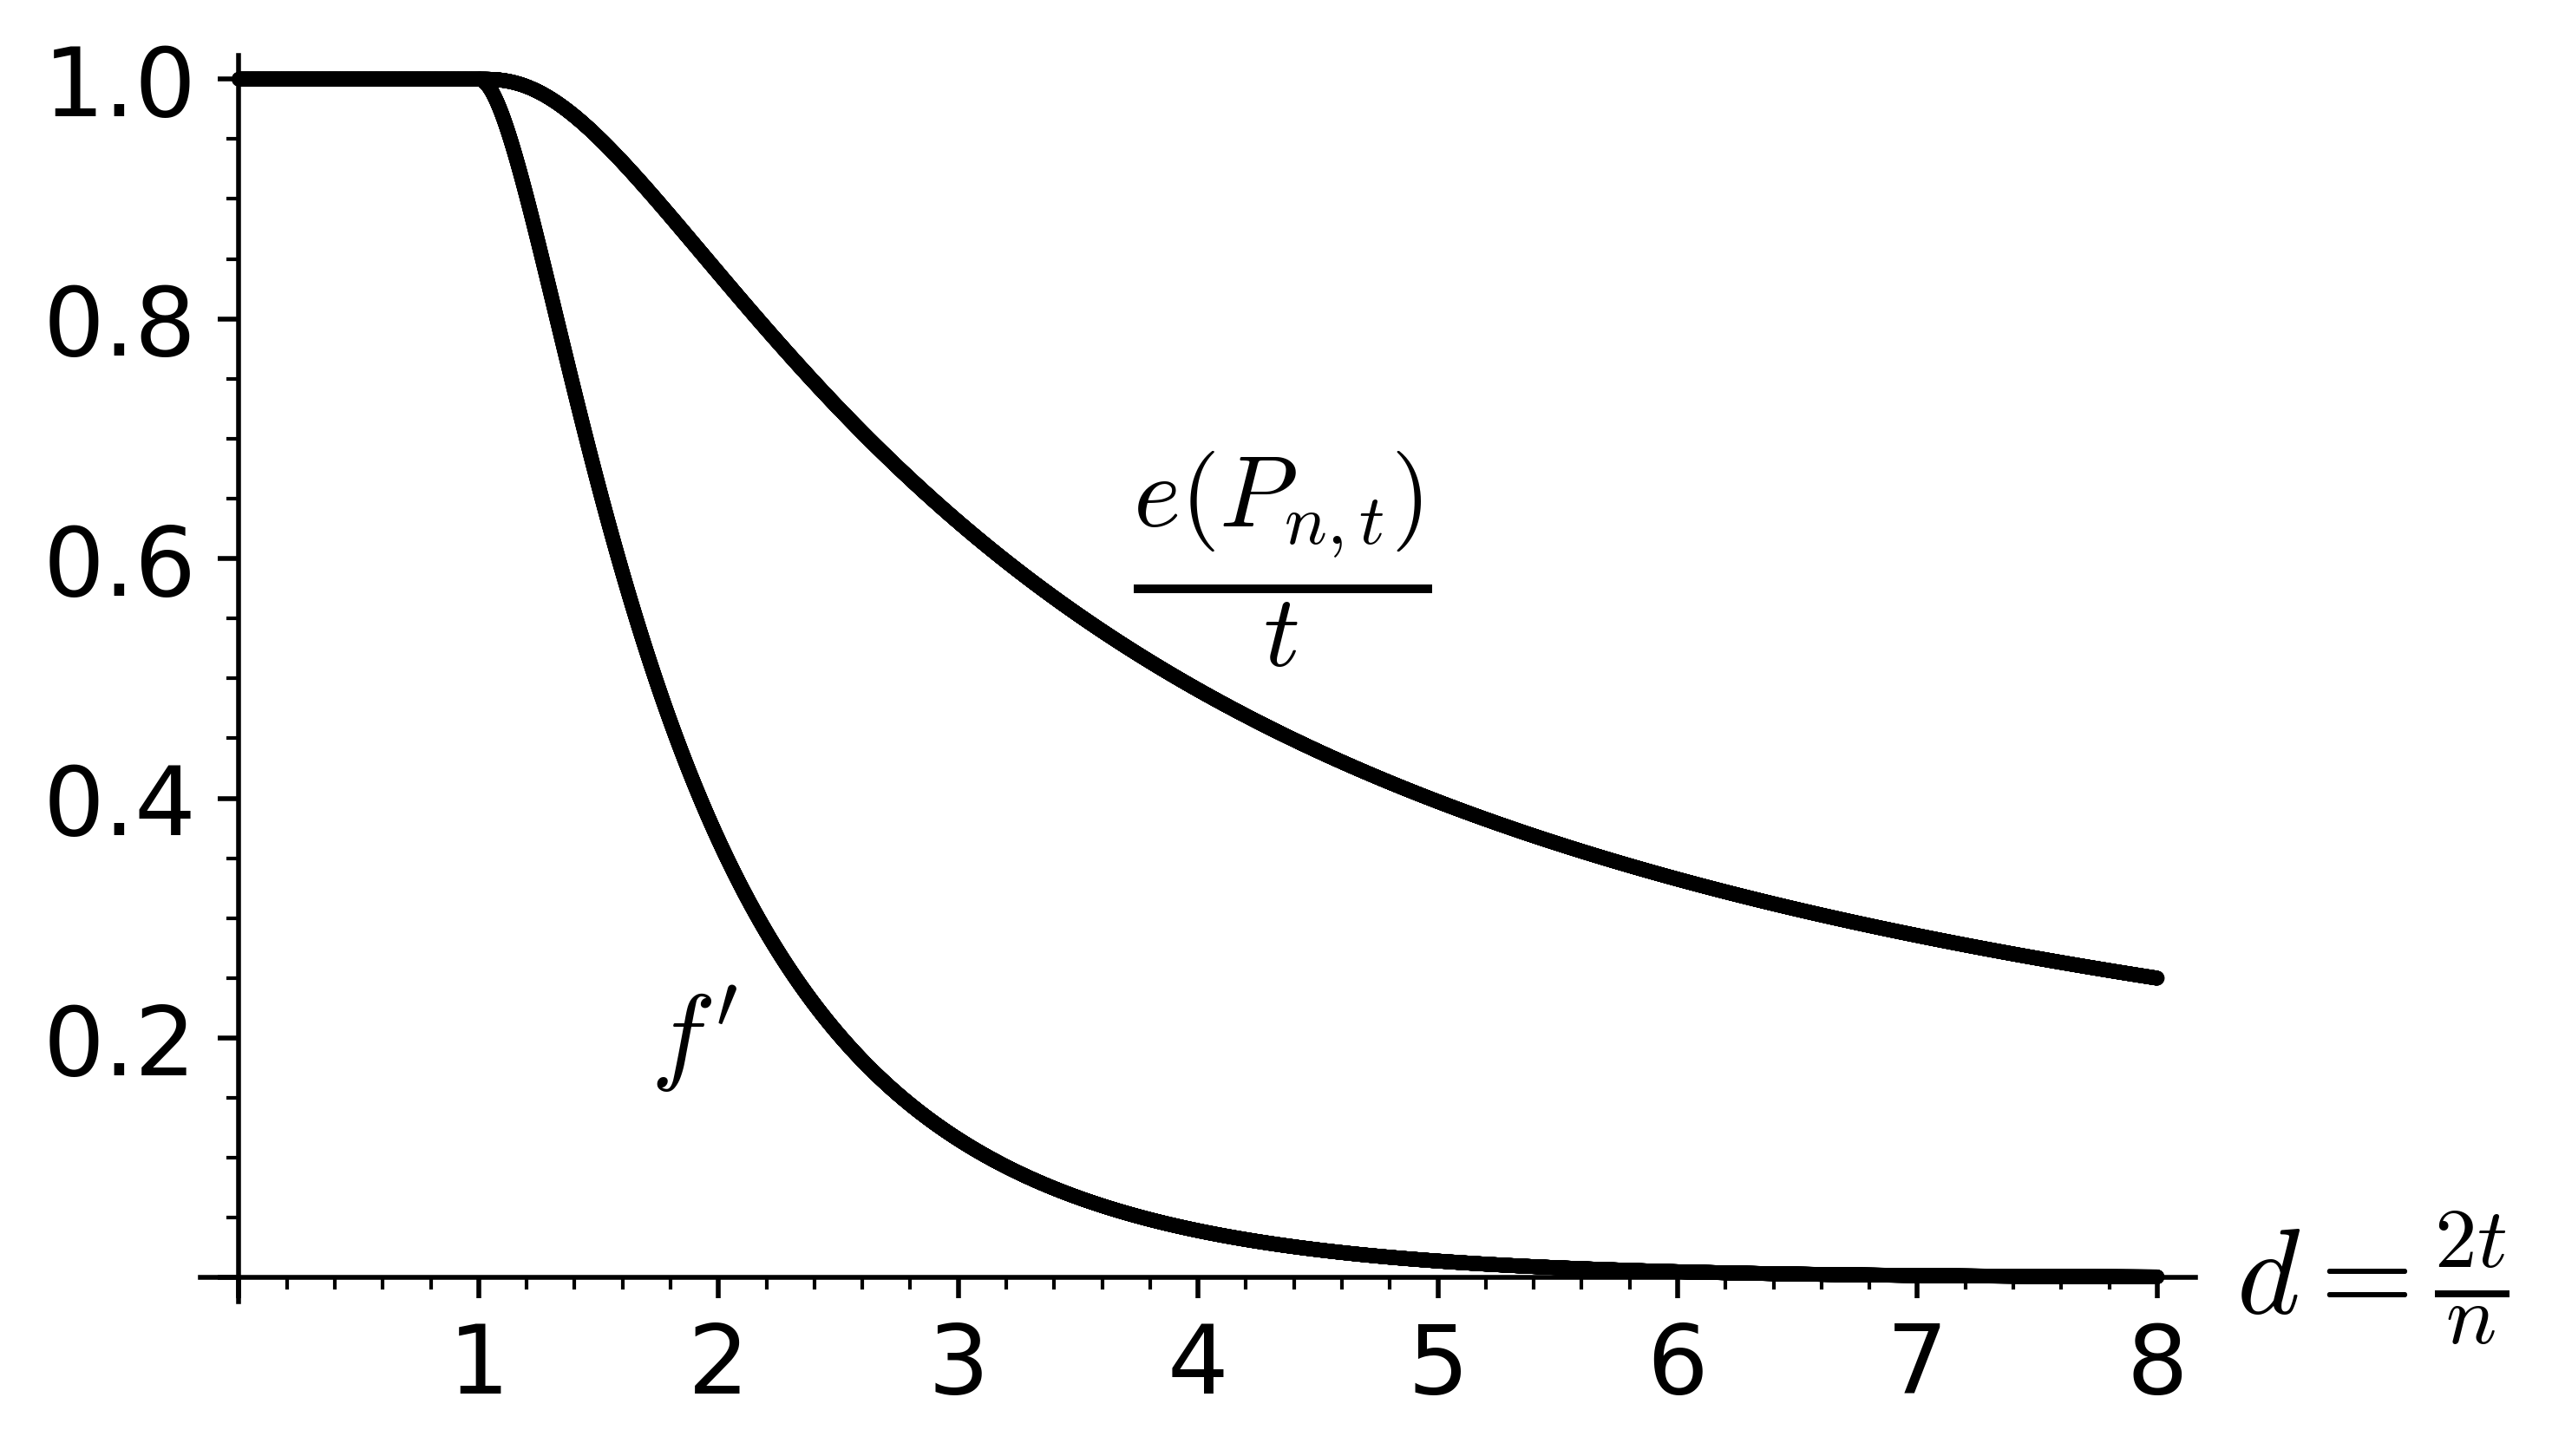
\includegraphics[scale=0.505]{process.png}
	\caption{The fraction $\numberEdges{\pro{n}{t}}/t$ of edges that are accepted up to step $t=dn/2$ and the derivative $f'(d)$ which equals the asymptotic probability that the edge in step $t=dn/2$ is accepted.}
	\label{fig:process}
\end{figure}

We refer to \Cref{fig:process} for an illustration of \Cref{thm:main_process_number_edges}. A generalisation of \Cref{thm:main_process_number_edges} to various other graph classes can be found in \Cref{PPthm:main}. Furthermore, \Cref{thm:main_process_number_edges} can be used to prove the following behaviour of the random planar graph process in step $t+1$ when $t=dn/2$ for a constant $d>1$: The considered edge is \lq typically\rq\ rejected if both endpoints lie in the largest component of $\pro{n}{t}$ and otherwise, it is accepted. 

Next, we consider the random graph $\acc{n}{m_0}$, which is the graph when exactly $m_0$ many edges have been {\em accepted} in the random planar graph process. More precisely, we are interested in the number of vertices $\numberVertices{L\left(\acc{n}{m_0}\right)}$ in the largest component of $\acc{n}{m_0}$. Gerke, Schlatter, Steger, and Taraz \cite{GerkeSchlatterStegerTaraz2008} proved that if $m_0=dn/2$ for a constant $d\in(2,6)$, whp $\acc{n}{m_0}$ is connected, i.e., whp $\numberVertices{L\left(\acc{n}{m_0}\right)}=n$. In the case $m_0\leq n/2+\bigo{n^{2/3}}$, the asymptotic behaviour of $\numberVertices{L\left(\acc{n}{m_0}\right)}$ can again be determined by using corresponding results on $\er{n}{t}$ (see \Cref{PPthm:largestComponent} for details). Hence, we focus on the regime $m_0=n/2+s$ for $s^3n^{-2}\to\infty$ and $s\leq n/2$. We denote by $f^{-1}$ the inverse of the function $f$ defined in \eqref{eq:2}. The next result provides the asymptotic order of the number of vertices in the largest component of $\acc{n}{m_0}$ and is a special case of \Cref{PPthm:largestComponent}.

\begin{thm}\label{thm:process_largest_component}
Whp the number $\numberVertices{L\left(\acc{n}{m_0}\right)}$ of vertices in the largest component of $\acc{n}{m_0}$ satisfies the following.
\begin{align*}
\numberVertices{L\left(\acc{n}{m_0}\right)}=
\begin{cases}
\left(4+\smallo{1}\right)s& \text{if} ~~ m_0=n/2+s ~~\text{for}~~ s^3n^{-2}\to \infty, s=\smallo{n};
\\
\left(\beta_{f^{-1}(d)}+\smallo{1}\right)n& \text{if} ~~ m_0=dn/2 ~~\text{for}~~ 1<d<2;
\\
\left(1+\smallo{1}\right)n& \text{if} ~~ m_0=dn/2 ~~\text{for}~~ d=2.
\end{cases}
\end{align*}
\end{thm}

Kang and \Luczak\ \cite{KangLuczak2012} showed that if $m_0=dn/2$ for a constant $d\in(1,2)$, then whp the largest component in the random planar graph $P\left(n,m_0\right)$ has $(d-1+\smallo{n})$ many vertices. Together with \Cref{thm:process_largest_component} and the fact that $\beta_{f^{-1}(d)}>\left(d-1\right)$ we have that the largest component in $\acc{n}{m_0}$ is typically much bigger than in $P\left(n,m_0\right)$.


\section{Key techniques and concepts}\label{sec:key_technique}

In this section we present our main approaches and ideas for studying the random planar graph $P=P(n,m)$.

In the so-called {\em core-kernel approach}, which was introduced by \Bollobas\ \cite{Bollobas1984b} and \Luczak\ \cite{Luczak1991b}, we construct $P$ stepwise by using simple operations, such as subdividing edges or replacing vertices by rooted trees. In \Cref{sub:decomposition_construction} we obtain the desired construction by reversing a decomposition of graphs. Subsequently in \Cref{sub:conditional_random_graphs}, we consider the concept of {\em conditional random graphs}, which allows us to study each construction step \lq almost\rq\ independently of the others and to transfer properties from them to the whole graph $P$. In \Cref{sub:random_complex_part,sub:random_kernel,sub:random_core,sub:random_noncomplex_part} we deal with each construction step in more detail and connections to well-known random experiments, such as the P\'olya urn or the balls-into-bins model. In \Cref{sub:largest_component} we demonstrate how to translate results obtained by the core-kernel approach to properties of the largest component and the remaining part of $P$. Finally in \Cref{sub:other_classes}, we discuss a generalisation of the core-kernel approach to various other graph classes.

\subsection{Decomposition and construction of graphs}\label{sub:decomposition_construction}
In this subsection we first introduce a decomposition of graphs into substructures, which we then reverse to construct the random planar graph $P(n,m)$. Finally, we explain how this construction leads to asymptotic results on $P(n,m)$.

In each of various steps of decomposition we extract a \lq smaller\rq\ substructure of the current graph such that the (non-)planarity of the graph is preserved. More precisely, given a (not necessarily planar) graph $H$, we obtain the {\em complex part} $\complexPart{H}$ of $H$ by removing the {\em non-complex part} $U(H)$, which is the union of all components of $H$ with at most one cycle. The {\em 2-core} $\core{H}$ of $H$ is the maximal subgraph of $\complexPart{H}$ with minimum degree at least two. Equivalently, the 2-core $\core{H}$ can be constructed by deleting recursively vertices of degree one in $\complexPart{H}$. We call a path in $\core{H}$ {\em maximal bare} if all its internal vertices have degree two (in $\core{H}$) and its endvertices are of degree at least three. Such a \lq path\rq\ is a cycle containing exactly one vertex with degree at least three if its endpoints are identical. We obtain the {\em kernel} $\kernel{H}$ of $H$ by replacing each maximal bare path in $\core{H}$ by an edge between the endpoints of the path, i.e., we remove all edges and internal vertices of the path and add instead an edge between the endpoints. In this decomposition step loops and multiple edges can appear, i.e., $\kernel{H}$ is a multigraph in general. We note that a graph is planar if and only if its kernel is.

Reversing this decomposition we can construct a graph $H$ as follows (see \Cref{fig:construction} for an illustration): We start with some multigraph with minimum degree at least three for the kernel $\kernel{H}$. Then we subdivide the edges of the kernel with additional vertices such that all loops and multiple edges are destroyed and to obtain the 2-core $\core{H}$. In the next step, we replace each vertex of the 2-core by a rooted tree to get the complex part $\complexPart{H}$. Finally, we add components with at most one cycle and end up with the graph $H$.


\def\shiftXa{15.6}
\def\shiftYa{0}
\def\shiftXb{10.4}
\def\shiftYb{0}
\def\shiftXc{5.2}
\def\shiftYc{0}
\def\shiftXd{0}
\def\shiftYd{0}

\begin{figure}[t]
\centering
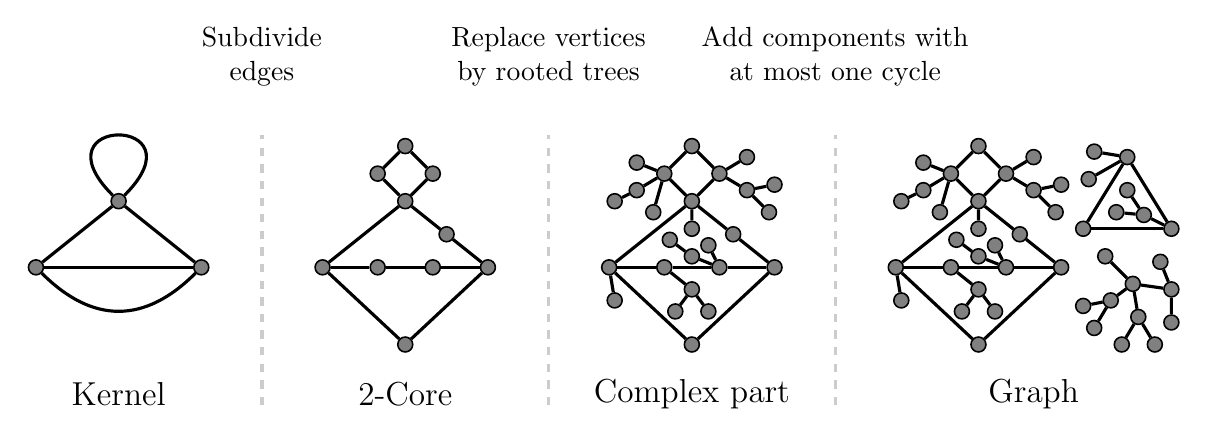
\begin{tikzpicture}[scale=0.7, line width=0.4mm, every node/.style={circle,fill=gray,draw,line width=0.2mm,inner sep=0,minimum size=0.19cm}]
\node (A) at (0+\shiftXa,0+\shiftYa) [draw]  {};
\node (A1) at (0.1+\shiftXa,-0.6+\shiftYa) [draw]  {};	
\node (B) at (1+\shiftXa,0+\shiftYa) [draw]  {};
\node (B1) at (1.5+\shiftXa,-0.4+\shiftYa) [draw]  {};
\node (B2) at (1.2+\shiftXa,-0.8+\shiftYa) [draw]  {};	
\node (B3) at (1.8+\shiftXa,-0.8+\shiftYa) [draw]  {};			
\node (C) at (2+\shiftXa,0+\shiftYa) [draw]  {};	
\node (C1) at (1.5+\shiftXa,0.2+\shiftYa) [draw]  {};	
\node (C2) at (1.8+\shiftXa,0.4+\shiftYa) [draw]  {};	
\node (C3) at (1.1+\shiftXa,0.5+\shiftYa) [draw]  {};	
\node (D) at (3+\shiftXa,0+\shiftYa) [draw]  {};
\node (E) at (1.5+\shiftXa,-1.4+\shiftYa) [draw]  {};	
\node (F) at (1.5+\shiftXa,1.2+\shiftYa) [draw]  {};	
\node (F1) at (1.5+\shiftXa,0.7+\shiftYa) [draw]  {};
\node (G) at (2.25+\shiftXa,0.6+\shiftYa) [draw]  {};	
\node (H) at (1.5+\shiftXa,2.2+\shiftYa) [draw]  {};
\node (I) at (1+\shiftXa,1.7+\shiftYa) [draw]  {};
\node (I1) at (0.5+\shiftXa,1.9+\shiftYa) [draw]  {};
\node (I2) at (0.5+\shiftXa,1.4+\shiftYa) [draw]  {};
\node (I3) at (0.8+\shiftXa,1+\shiftYa) [draw]  {};
\node (I4) at (0.1+\shiftXa,1.2+\shiftYa) [draw]  {};	
\node (J) at (2+\shiftXa,1.7+\shiftYa) [draw]  {};
\node (J1) at (2.5+\shiftXa,1.4+\shiftYa) [draw]  {};
\node (J2) at (2.5+\shiftXa,2+\shiftYa) [draw]  {};
\node (J3) at (2.9+\shiftXa,1+\shiftYa) [draw]  {};
\node (J4) at (3+\shiftXa,1.5+\shiftYa) [draw]  {};

\draw[-] (A) to (B);
\draw[-] (B) to (C);
\draw[-] (C) to (D);
\draw[-] (A) to (E);
\draw[-] (D) to (E);
\draw[-] (B) to (B1);
\draw[-] (B1) to (B2);
\draw[-] (B1) to (B3);	
\draw[-] (D) to (G);
\draw[-] (F) to (G);
\draw[-] (A) to (F);
\draw[-] (F) to (I);
\draw[-] (F) to (J);
\draw[-] (H) to (I);
\draw[-] (H) to (J);
\draw[-] (C) to (C1);
\draw[-] (C) to (C2);
\draw[-] (C1) to (C3);	
\draw[-] (A) to (A1);
\draw[-] (J) to (J1);
\draw[-] (J) to (J2);
\draw[-] (J1) to (J3);
\draw[-] (J1) to (J4);
\draw[-] (F) to (F1);
\draw[-] (I) to (I1);
\draw[-] (I) to (I2);
\draw[-] (I) to (I3);
\draw[-] (I2) to (I4);	

\node (K) at (3.4+\shiftXa,0.7+\shiftYa) [draw]  {};
\node (L) at (5+\shiftXa,0.7+\shiftYa) [draw]  {};
\node (M) at (4.2+\shiftXa,2+\shiftYa) [draw]  {};
\node (L1) at (4.5+\shiftXa,0.95+\shiftYa) [draw]  {};
\node (L2) at (4.2+\shiftXa,1.4+\shiftYa) [draw]  {};
\node (L3) at (4+\shiftXa,1+\shiftYa) [draw]  {};
\node (M1) at (3.6+\shiftXa,2.1+\shiftYa) [draw]  {};
\node (M2) at (3.5+\shiftXa,1.6+\shiftYa) [draw]  {};
\node (N1) at (4.3+\shiftXa,-0.3+\shiftYa) [draw]  {};
\node (N2) at (5+\shiftXa,-0.4+\shiftYa) [draw]  {};
\node (N3) at (4.4+\shiftXa,-0.9+\shiftYa) [draw]  {};
\node (N4) at (4.1+\shiftXa,-1.4+\shiftYa) [draw]  {};
\node (N5) at (4.7+\shiftXa,-1.4+\shiftYa) [draw]  {};
\node (N6) at (3.8+\shiftXa,0.2+\shiftYa) [draw]  {};
\node (N7) at (5+\shiftXa,-1+\shiftYa) [draw]  {};
\node (N8) at (4.8+\shiftXa,0.1+\shiftYa) [draw]  {};
\node (N9) at (3.9+\shiftXa,-0.6+\shiftYa) [draw]  {};
\node (N10) at (3.4+\shiftXa,-0.7+\shiftYa) [draw]  {};	
\node (N11) at (3.6+\shiftXa,-1.1+\shiftYa) [draw]  {};	

\node () at (2.5+\shiftXa,-2.3+\shiftYa) [fill=none, rectangle, draw=none, align=center]  {\large Graph};
\draw[-] (K) to (L);
\draw[-] (K) to (M);	
\draw[-] (L) to (M);	
\draw[-] (L) to (L1);	
\draw[-] (L1) to (L2);	
\draw[-] (L1) to (L3);	
\draw[-] (M) to (M1);	
\draw[-] (M) to (M2);	
\draw[-] (N1) to (N2);	
\draw[-] (N1) to (N3);	
\draw[-] (N3) to (N4);	
\draw[-] (N3) to (N5);	
\draw[-] (N1) to (N6);	
\draw[-] (N2) to (N7);	
\draw[-] (N2) to (N8);
\draw[-] (N1) to (N9);	
\draw[-] (N9) to (N10);	
\draw[-] (N9) to (N11);

\draw[-,dashed,gray,opacity=0.4] (14.5,-2.5) to (14.5,2.4);

%Complex part
\node (A) at (0+\shiftXb,0+\shiftYb) [draw]  {};
\node (A1) at (0.1+\shiftXb,-0.6+\shiftYb) [draw]  {};	
\node (B) at (1+\shiftXb,0+\shiftYb) [draw]  {};
\node (B1) at (1.5+\shiftXb,-0.4+\shiftYb) [draw]  {};
\node (B2) at (1.2+\shiftXb,-0.8+\shiftYb) [draw]  {};
\node (B3) at (1.8+\shiftXb,-0.8+\shiftYb) [draw]  {};
\node (C) at (2+\shiftXb,0+\shiftYb) [draw]  {};
\node (C1) at (1.5+\shiftXb,0.2+\shiftYb) [draw]  {};	
\node (C2) at (1.8+\shiftXb,0.4+\shiftYb) [draw]  {};	
\node (C3) at (1.1+\shiftXb,0.5+\shiftYb) [draw]  {};	
\node (D) at (3+\shiftXb,0+\shiftYb) [draw]  {};
\node (E) at (1.5+\shiftXb,-1.4+\shiftYb) [draw]  {};	
\node (F) at (1.5+\shiftXb,1.2+\shiftYb) [draw]  {};	
\node (F1) at (1.5+\shiftXb,0.7+\shiftYb) [draw]  {};
\node (G) at (2.25+\shiftXb,0.6+\shiftYb) [draw]  {};	
\node (H) at (1.5+\shiftXb,2.2+\shiftYb) [draw]  {};
\node (I) at (1+\shiftXb,1.7+\shiftYb) [draw]  {};
\node (I1) at (0.5+\shiftXb,1.9+\shiftYb) [draw]  {};
\node (I2) at (0.5+\shiftXb,1.4+\shiftYb) [draw]  {};
\node (I3) at (0.8+\shiftXb,1+\shiftYb) [draw]  {};
\node (I4) at (0.1+\shiftXb,1.2+\shiftYb) [draw]  {};	
\node (J) at (2+\shiftXb,1.7+\shiftYb) [draw]  {};
\node (J1) at (2.5+\shiftXb,1.4+\shiftYb) [draw]  {};
\node (J2) at (2.5+\shiftXb,2+\shiftYb) [draw]  {};
\node (J3) at (2.9+\shiftXb,1+\shiftYb) [draw]  {};
\node (J4) at (3+\shiftXb,1.5+\shiftYb) [draw]  {};
\node () at (1.5+\shiftXb,-2.3+\shiftYb) [fill=none, rectangle, draw=none, align=center]  {\large Complex part};

\draw[-] (A) to (B);
\draw[-] (B) to (C);
\draw[-] (C) to (D);
\draw[-] (A) to (E);
\draw[-] (D) to (E);
\draw[-] (B) to (B1);
\draw[-] (B1) to (B2);
\draw[-] (B1) to (B3);	
\draw[-] (D) to (G);
\draw[-] (F) to (G);
\draw[-] (A) to (F);
\draw[-] (F) to (I);
\draw[-] (F) to (J);
\draw[-] (H) to (I);
\draw[-] (H) to (J);
\draw[-] (C) to (C1);
\draw[-] (C) to (C2);
\draw[-] (C1) to (C3);	
\draw[-] (A) to (A1);
\draw[-] (J) to (J1);
\draw[-] (J) to (J2);
\draw[-] (J1) to (J3);
\draw[-] (J1) to (J4);
\draw[-] (F) to (F1);
\draw[-] (I) to (I1);
\draw[-] (I) to (I2);
\draw[-] (I) to (I3);
\draw[-] (I2) to (I4);

\node () at (4.1+\shiftXb,3.5+\shiftYb) [fill=none, rectangle, draw=none, align=center]  {Add components with\\  at most one cycle\\[0.1cm] {\huge \MVRightarrow}};

%Core
\node (A) at (0+\shiftXc,0+\shiftYc) [draw]  {};	
\node (B) at (1+\shiftXc,0+\shiftYc) [draw]  {};		
\node (C) at (2+\shiftXc,0+\shiftYc) [draw]  {};	
\node (D) at (3+\shiftXc,0+\shiftYc) [draw]  {};
\node (E) at (1.5+\shiftXc,-1.4+\shiftYc) [draw]  {};	
\node (F) at (1.5+\shiftXc,1.2+\shiftYc) [draw]  {};	
\node (G) at (2.25+\shiftXc,0.6+\shiftYc) [draw]  {};	
\node (H) at (1.5+\shiftXc,2.2+\shiftYc) [draw]  {};
\node (I) at (1+\shiftXc,1.7+\shiftYc) [draw]  {};
\node (J) at (2+\shiftXc,1.7+\shiftYc) [draw]  {};
\node () at (1.5+\shiftXc,-2.3+\shiftYc) [fill=none, rectangle, draw=none, align=center]  {\large 2-Core};

\draw[-] (A) to (B);
\draw[-] (B) to (C);
\draw[-] (C) to (D);
\draw[-] (A) to (E);
\draw[-] (D) to (E);	
\draw[-] (D) to (G);
\draw[-] (F) to (G);
\draw[-] (A) to (F);
\draw[-] (F) to (I);
\draw[-] (F) to (J);
\draw[-] (H) to (I);
\draw[-] (H) to (J);

\draw[-,dashed,gray,opacity=0.4] (9.3,-2.5) to (9.3,2.4);

\node () at (9.3,3.5+\shiftYc) [fill=none, rectangle, draw=none, align=center]  {Replace vertices\\ by rooted trees\\[0.1cm] {\huge \MVRightarrow}};

%Kernel
\node (A) at (0+\shiftXd,0+\shiftYd) [draw]  {};		
\node (D) at (3+\shiftXd,0+\shiftYd) [draw]  {};
\node (F) at (1.5+\shiftXd,1.2+\shiftYd) [draw]  {};	
\node () at (1.5,-2.3+\shiftYd) [fill=none, rectangle, draw=none, align=center]  {\large Kernel};

\draw[-,dashed,gray,opacity=0.4] (4.1,-2.5) to (4.1,2.4);

\node () at (4.1,3.5+\shiftYd) [fill=none, rectangle, draw=none, align=center] {Subdivide\\ edges\\[0.1cm] {\huge \MVRightarrow}};
			
\draw[-] (A) to (D);	
\draw[-] (D) to (F);
\draw[-] (A) to (F);
\draw (F) to [out=45,in=135,looseness=25] (F);	
\draw (A) to [out=315,in=225,looseness=1.2] (D);

\end{tikzpicture}
\caption{Construction of a graph in the core-kernel approach: We start with the kernel and subdivide its edges to obtain the 2-core. Then we replace each vertex by a rooted tree to get the complex part. Finally, we end up with the graph by adding components with at most one cycle.}
\label{fig:construction}
\end{figure}

This construction of graphs motivates to sample the random planar graph $P=P(n,m)$ by revealing the following parts one after another:
\begin{enumerate}[label={(C\arabic*)}]
    \item\label{con:step1} Vertex set $\vertexSet{\kernel{P}}$ of the kernel and the number $\numberEdges{\kernel{P}}$ of edges in the kernel;
    \item\label{con:step2} Kernel $\kernel{P}$ by choosing a random multigraph on vertex set $\vertexSet{\kernel{P}}$ with $\numberEdges{\kernel{P}}$ edges;
    \item\label{con:step3} Vertex set $\vertexSet{\core{P}}$ of the 2-core;
    \item\label{con:step4} 2-Core $\core{P}$ by randomly subdividing the edges of $\kernel{P}$ with the vertices in $\vertexSet{\core{P}}\setminus\vertexSet{\kernel{P}}$ such that all loops and multiple edges are destroyed;
    \item\label{con:step5} Vertex set $\vertexSet{\complexPart{P}}$ of the complex part;
    \item\label{con:step6} Complex part $\complexPart{P}$ by randomly replacing each vertex of $\core{P}$ by a rooted tree such that the vertex set of the union of the trees is $\vertexSet{\complexPart{P}}$;
    \item\label{con:step7} The random planar graph $P$ by randomly adding components with at most one cycle on vertex set $[n]\setminus\vertexSet{\complexPart{P}}$
    having in total $m+\numberVertices{\kernel{P}}-\numberVertices{\complexPart{P}}-\numberEdges{\kernel{P}}$ edges.
\end{enumerate}

We note that the random operations in \ref{con:step2}, \ref{con:step4}, \ref{con:step6}, and \ref{con:step7} do not necessarily obey the uniform distribution, e.g., not every multigraph with vertex set $\vertexSet{\kernel{P}}$ and $\numberEdges{\kernel{P}}$ edges is equally likely to be obtained in \ref{con:step2}.

The generic idea of the core-kernel approach is to determine for every construction step properties which hold whp after performing this step. We call them for short {\em whp-properties} and typical examples are that a revealed vertex set is of certain size or that the length of the longest cycle in an obtained (multi)graph is of certain asymptotic order. We note that whp-properties for the final construction step \ref{con:step7} lead to asymptotic results on the random planar graph $P$. Roughly speaking, we can split the ways of obtaining whp-properties into two different types.

\begin{itemize}
    \item Type I: In steps \ref{con:step1}, \ref{con:step3}, and \ref{con:step5}, we are mostly interested in the sizes of the revealed vertex sets rather than the precise labels of the vertices. Therefore, the whp-properties we use for these steps are results on the asymptotic orders of $\numberVertices{\kernel{P}}$, $\numberEdges{\kernel{P}}$, $\numberVertices{\core{P}}$, and $\numberVertices{\complexPart{P}}$ from \cite{KangLuczak2012,KangMosshammerSpruessel2020}.
    \item Type II: For the remaining steps \ref{con:step2}, \ref{con:step4}, \ref{con:step6}, and \ref{con:step7} we analyse how they \lq change\rq\ the whp-properties obtained in the previous steps, e.g., how they change the cycle structure or the maximum degree of a (multi)graph. For instance, assume that we already know that whp the kernel $\kernel{P}$ (after \ref{con:step2}) and the vertex set $\vertexSet{\core{P}}$ (in \ref{con:step3}) fulfil a certain property $\mathcal{T}$ and that we want to show that whp the 2-core $\core{P}$ (after \ref{con:step4}) satisfies property $\property$. We aim to show that whenever we condition on realisations of $\kernel{P}$ and $\vertexSet{\core{P}}$ that satisfy $\mathcal{T}$, whp $\property$ is true after performing (C4). This would imply that whp $\property$ holds also in the 2-core $\core{P}$, i.e., we would obtain a property of the \lq unconditional\rq\ 2-core $\core{P}$ (where $\kernel{P}$ and $\vertexSet{\core{P}}$ are random) by investigating only \lq conditional\rq\ 2-cores (where $\kernel{P}$ and $\vertexSet{\core{P}}$ are fixed). In \Cref{sub:conditional_random_graphs} we provide a general framework for this \lq conditional\rq\ random graphs and a formal statement which can be used to transfer properties to \lq unconditional\rq\ random graphs (see \Cref{lem:cond_graph}). 
\end{itemize}

We analyse \ref{con:step2}, \ref{con:step4}, \ref{con:step6}, and \ref{con:step7} for fixed realisations of the previous steps in more detail in \Cref{sub:random_complex_part,sub:random_core,sub:random_kernel,sub:random_noncomplex_part}. In particular, we provide useful relations between the steps \ref{con:step4}, \ref{con:step6}, and \ref{con:step7} and the P\'olya urn model, the balls-into-bins model, and the critical \ER\ random graph, respectively. These connections allow us to obtain really strong properties of $\core{P}$, $\complexPart{P}$, and $P$, which seems to be quite difficult when studying these random graphs \lq directly\rq. 

To sum up, we have the following \lq generic plan\rq\ for determining asymptotic properties of the random planar graph $P$: We start with results on the asymptotic number of vertices and edges in the kernel due to Kang and \Luczak\ \cite{KangLuczak2012} and Kang, Mo{\ss}hammer, and Spr\"{u}ssel \cite{KangMosshammerSpruessel2020}. Then we apply double counting arguments to obtain whp-properties of the kernel $\kernel{P}$ (see \Cref{sub:random_kernel} for details). Using them and statements on the asymptotic number of vertices in the 2-core from \cite{KangLuczak2012,KangMosshammerSpruessel2020} as an \lq input\rq\ of a P\'olya urn model, leads to whp-properties of the 2-core $\core{P}$ (see \Cref{sub:random_core} for details). These whp-properties and results on the asymptotic number of vertices in the complex part due to \cite{KangLuczak2012,KangMosshammerSpruessel2020} are then the main \lq ingredients\rq\ for a balls-into-bins model, which provides whp-properties of the complex part $\complexPart{P}$ (see \Cref{sub:random_complex_part} for details). Because whp-properties of the non-complex part $U(P)$ follow from well-known results on the critical \ER\ random graph, combining them with whp-properties of the complex part $\complexPart{P}$ allows us to obtain whp-properties of $P$ (see \Cref{sub:random_noncomplex_part} for details). This core-kernel approach is illustrated in \Cref{fig:overview}.

\begin{figure}[t]
\centering
\begin{tikzpicture}[scale=0.8, line width=0.4mm]
\node (A) at (0,-0.5) [draw]  {Results from \cite{KangLuczak2012} and \cite{KangMosshammerSpruessel2020}};
\node (B) at (-6,-3) [draw, align=left]{\ref{con:step1}: Asymptotic \\  number of vertices and\\ edges in the kernel};
\node (C) at (0.5,-3) [draw, align=left]{\ref{con:step3}: Asymptotic\\  number of vertices\\ in the 2-core};
\node (D) at (6.5,-3) [draw, align=left]{\ref{con:step5}: Asymptotic\\ number of vertices\\ in the complex part};
\draw[->] (A) to (-6,-1.98);
\draw[->] (A) to (C);
\draw[->] (A) to (6,-1.98);
\node (E) at (-6,-4.7) [draw, circle, inner sep=0.1mm]{+};
\node (F) at (-6,-6) [draw, ellipse, align=left, inner xsep=-2mm, inner ysep=1.5mm]{Double counting};
%\node (G) at (-6,-7.3) [draw, circle, inner sep=0.5mm]{=};
\node (H) at (-6,-8) [draw, align=left]{\ref{con:step2}: Properties of kernel};
\draw[-] (B) to (E);
\draw[-] (E) to (F);
%\draw[-] (F) to (G);
\draw[->] (F) to (H);
\node (I) at (0.5,-5.8) [draw, circle, inner sep=0.1mm]{+};
\node (J) at (-1.85,-8) [draw, circle, inner sep=0.1mm]{+};
\node (K) at (0.5,-8) [draw, ellipse, align=left, inner xsep=-1mm, inner ysep=1.5mm]{P\'olya urn};
%\node (L) at (0.5,-9.8) [draw, circle, inner sep=0.5mm]{=};
\node (M) at (0.5,-10) [draw, align=left]{\ref{con:step4}: Properties of 2-core};
\draw[-] (C) to (I);
\draw[-] (I) to (K);
\draw[-] (H) to (J);
\draw[-] (J) to (K);
%\draw[-] (K) to (L);
\draw[->] (K) to (M);

\node (N) at (6.5,-6.85) [draw, circle, inner sep=0.1mm]{+};
\node (O) at (3.975,-10) [draw, circle, inner sep=0.1mm]{+};
\node (P) at (6.5,-10) [draw, ellipse, align=left, inner xsep=-1mm, inner ysep=1.5mm]{Balls into bins};
%\node (Q) at (6.5,-12.1) [draw, circle, inner sep=0.5mm]{=};
\node (R) at (6.5,-12) [draw, align=left]{\ref{con:step6}: Properties \\of complex part};
\draw[-] (D) to (N);
\draw[-] (N) to (P);
\draw[-] (M) to (O);
\draw[-] (O) to (P);
%\draw[-] (P) to (Q);
\draw[->] (P) to (R);

\node (S) at (2.85,-12.5) [draw, circle, inner sep=0.1mm]{+};
\node (T) at (-3,-13.25) [draw, align=left]{Critical \ER\ random graph: \\Properties of non-complex part};
%\node (U) at (2.6,-15.5) [draw, circle, inner sep=0.5mm]{=};
\node (V) at (6.5,-14.5) [draw, align=left]{\ref{con:step7}: Properties of\\ random planar graph};
\draw[-] (R) to (S);
\draw[-] (S) to (T);
%\draw[-] (T) to (U);
\draw[->] (T) to (V);

\end{tikzpicture}
\caption{Overview of the core-kernel approach.}
\label{fig:overview}
\end{figure}

%\begin{figure}[t]
%\centering
%\begin{tikzpicture}[scale=0.8, line width=0.4mm, every node/.style={circle,draw,line width=0.35mm,inner sep=0.03cm,minimum size=0.38cm, fill=gray, fill opacity=0.3, text opacity=1}]
%\node (A) at (0,0) [draw]  {\scriptsize \textbf{3}};
%\node (B) at (1,0) [draw]  {\scriptsize \textbf{4}};
%\node (C) at (0,1) [draw]  {\scriptsize \textbf{1}};
%\node (D) at (1,1) [draw]  {\scriptsize \textbf{2}};

%\node (E) at (2,1.1) [draw, minimum size=0.17cm, fill opacity=1]  {};
%\node (F) at (2.8,1.1) [draw, minimum size=0.17cm, fill opacity=1]  {};
%\node (G) at (2,0.7) [draw, minimum size=0.17cm, fill opacity=1]  {};
%\node (H) at (2.8,0.7) [draw, minimum size=0.17cm, fill opacity=1]  {};
%\node (I) at (2,0.3) [draw, minimum size=0.17cm, fill opacity=1]  {};
%\node (J) at (2.8,0.3) [draw, minimum size=0.17cm, fill opacity=1]  {};
%\node (K) at (2,-0.1) [draw, minimum size=0.17cm, fill opacity=1]  {};
%\node (L) at (2.8,-0.1) [draw, minimum size=0.17cm, fill opacity=1]  {};
%\node (M) at (3.3,0.1) [draw, minimum size=0.17cm, fill opacity=1]  {};
%\node (N) at (3.3,0.9) [draw, minimum size=0.17cm, fill opacity=1]  {};
%\node (O) at (3.8,0.1) [draw, minimum size=0.17cm, fill opacity=1]  {};
%\node (P) at (3.8,0.9) [draw, minimum size=0.17cm, fill opacity=1]  {};

%\draw[-] (E) to (F);
%\draw[-] (G) to (H);
%\draw[-] (I) to (J);
%\draw[-] (K) to (L);
%\draw[-] (M) to (N);
%\draw[-] (O) to (P);

%\node () at (1.75,-1.5) [fill=none, rectangle, draw=none, align=left]  {\large %\ref{con:step1}:  Vertex set and \\number of edges of kernel};

%\draw[-,dashed,gray,opacity=0.4] (5,-2.2) to (5,1.3);

%\node (Q) at (7,-0.5) [draw]  {\scriptsize \textbf{3}};
%\node (R) at (6,1) [draw]  {\scriptsize \textbf{4}};
%\node (S) at (8,1) [draw]  {\scriptsize \textbf{1}};
%\node (T) at (9.2,0) [draw]  {\scriptsize \textbf{2}};

%\draw[-] (Q) to (R);
%\draw[-] (Q) to (S);
%\draw[-] (R) to (S);
%\draw[-] (S) to (T);
%\draw (T) to [out=315,in=45,looseness=20] (T);	
%\draw (Q) to [out=210,in=225,looseness=1] (R);

%\node () at (8.25,-1.75) [fill=none, rectangle, draw=none, align=left]  {\large %\ref{con:step2}: Kernel};

%\draw[-,dashed,gray,opacity=0.4] (11.5,-2.2) to (11.5,1.3);

%\node () at (13,-0.9) [draw]  {\tiny \textbf{13}};
%\node () at (14,-0.9) [draw]  {\tiny \textbf{14}};
%\node () at (15,-0.9) [draw]  {\tiny \textbf{15}};
%\node () at (16,-0.9) [draw]  {\tiny \textbf{16}};
%\node () at (13,-0.2) [draw]  {\scriptsize \textbf{9}};
%\node () at (14,-0.2) [draw]  {\tiny \textbf{10}};
%\node () at (15,-0.2) [draw]  {\tiny \textbf{11}};
%\node () at (16,-0.2) [draw]  {\tiny \textbf{12}};
%\node () at (13,0.5) [draw]  {\scriptsize \textbf{5}};
%\node () at (14,0.5) [draw]  {\scriptsize \textbf{6}};
%\node () at (15,0.5) [draw]  {\scriptsize \textbf{7}};
%\node () at (16,0.5) [draw]  {\scriptsize \textbf{8}};
%\node () at (13,1.2) [draw]  {\scriptsize \textbf{1}};
%\node () at (14,1.2) [draw]  {\scriptsize \textbf{2}};
%\node () at (15,1.2) [draw]  {\scriptsize \textbf{3}};
%\node () at (16,1.2) [draw]  {\scriptsize \textbf{4}};


%\node () at (14.5,-1.75) [fill=none, rectangle, draw=none, align=left]  {\large %\ref{con:step3}: Vertex set of 2-core};

%\end{tikzpicture}
%\caption{}
%\label{fig:overview}
%\end{figure}


To demonstrate how to apply the core-kernel approach in practise, here we sketch our strategy for determining the girth, i.e., the length of the shortest cycle, of the largest component $\largestcomponent{P}$ of $P=P(n,m)$ in the weakly supercritical regime when $m=n/2+s$ for $s^3n^{-2}\to \infty$ and $s=\smallo{n}$ (see \Cref{thm:main_cycle} for a formal statement and \Cref{CBproofof:thm:general} for its proof): Due to \cite{KangLuczak2012,KangMosshammerSpruessel2020}, we have in \ref{con:step1} that whp $\numberVertices{\kernel{P}}=\Th{sn^{-2/3}}$ and the kernel $\kernel{P}$ is cubic, thus, $\numberEdges{\kernel{P}}=3/2\numberVertices{\kernel{P}}$. Using double counting arguments we show that whp a cubic planar multigraph has linearly many loops. This implies that in \ref{con:step2} whp $\kernel{P}$ has $\Th{sn^{-2/3}}$ many loops. For \ref{con:step3} we use again results from \cite{KangLuczak2012,KangMosshammerSpruessel2020} to obtain that whp $\numberVertices{\core{P}}=\Th{sn^{-1/3}}$. Next, we show that for all fixed kernels and vertex sets of the 2-core, which satisfy the whp-properties obtained in the previous steps \ref{con:step1}--\ref{con:step3}, the following hold when we subdivide the edges of the kernel in \ref{con:step4}: Each edge is subdivided by $\OmegaP{ns^{-1}}$ vertices and because there are \lq many\rq\ loops, at least one loop is subdivided by $\ThetaP{ns^{-1}}$ vertices. In particular, this implies that the girth of the 2-core $\core{P}$ is of order $\ThetaP{ns^{-1}}$. We obtain these results by connecting the random subdivision of a kernel to the P\'olya urn model and analysing the minimum number of balls of the same colour in the urn (see \Cref{sub:random_core}). We observe that each cycle in the complex part is also contained in the 2-core. Thus, we immediately obtain that after steps \ref{con:step5} and \ref{con:step6} the girth of the complex part $\complexPart{P}$ is of order $\ThetaP{ns^{-1}}$. Finally, we show that whp the girth of the largest component coincides with the girth of the complex part (see \Cref{sub:largest_component} for details). Hence, after performing the final construction step \ref{con:step7} we get that the girth of $\largestcomponent{P}$ is of order $\ThetaP{ns^{-1}}$.

\subsection{Conditional random graphs}\label{sub:conditional_random_graphs}
Instead of analysing a random graph $A$ \lq directly\rq, we often want to consider $A$ conditioned on some properties it has. In the following definition we introduce a formal setting for these \lq conditional\rq\ random graphs. Given a class $\mathcal{A}$ of graphs and a positive integer $n\in\N$, we denote by $\mathcal{A}(n)\subseteq\mathcal{A}$ the subclass consisting of all graphs which have vertex set $[n]$.

\begin{definition}
Let $\cl$ be a class of graphs, $\mathcal{S}$ a set, and $\func:\cl\to \mathcal{S}$ a function. We say that a sequence $\seq=(s_n)_{n\in \N} \in \mathcal{S}^\N$ is {\em feasible} for $\left(\cl, \func\right)$ if for every $n \in \N$ there is a graph $H \in \cl(n)$ with $\func(H)=s_n$. We write $\left(\condGraph{\randomGraph}{\seq}\right)=\left(\condGraph{\randomGraph}{\seq}\right)(n)$ for a graph chosen uniformly at random from $\setbuilder{H \in \cl(n)}{\func(H)=s_n}$.
\end{definition}

Next, we provide a way to transfer properties from the conditional random graph $\left(\condGraph{\randomGraph}{\seq}\right)(n)$ to the random graph $A=A(n)$. We note that a graph property is just a set of graphs and therefore, we write $H\in \property$ if a graph $H$ fulfils the property $\property$.

\begin{lem}\label{lem:cond_graph}
Let $\cl$ be a class of graphs, $A=A(n)$ a graph chosen uniformly at random from $\mathcal{A}(n)$, $\mathcal{S}$ a set, and $\func:\cl\to \mathcal{S}$ a function. Assume that $\mathcal{T}\subseteq \mathcal{S}$ is a subset of $\mathcal{S}$ such that whp $\func(\randomGraph)\in \mathcal{T}$. Furthermore, let $\property$ be a graph property such that for every feasible sequence $\mathbf{t}\in \mathcal{T}^\N$, whp $\condGraph{\randomGraph}{\mathbf{t}} \in \property$. Then we have whp $\randomGraph \in \property$.
\end{lem}

We often apply \Cref{lem:cond_graph} in connection with the construction steps \ref{con:step1}--\ref{con:step7}. For example, to show that some property $\mathcal{Q}$ holds in the 2-core $\core{P}$ in \ref{con:step4} we typically use \Cref{lem:cond_graph} with the following quantities: For $\mathcal{A}(n)$ we choose the set of all planar graphs on vertex set $[n]$ having $m=m(n)$ edges. Moreover, we define the function $\func$ such that for each graph $H\in \mathcal{A}:=\bigcup_{n\in\N}\mathcal{A}(n)$ we have $\func(H)=\left(K(H), \vertexSet{\core{H}}\right)$. For $\mathcal{T}$ we use some property of the kernel $\kernel{P}$ and the vertex set $\vertexSet{\core{P}}$ which holds whp, e.g., $\numberVertices{\kernel{P}}$, $\numberEdges{\kernel{P}}$, and $\numberVertices{\core{P}}$ are of a certain asymptotic order. We typically attain such properties $\mathcal{T}$ via construction steps \ref{con:step1}--\ref{con:step3}. Then the main part is to show that for every feasible $\mathbf{t}\in\mathcal{T}^\N$, whp the 2-core of the conditional random graph $\condGraph{A}{\mathbf{t}}$ satisfies $\mathcal{Q}$. Finally, \Cref{lem:cond_graph} implies that whp $\property$ holds also in $\core{P}$.

We note that the idea of conditional random graphs is very elementary and is used quite often in literature. However, to the best of our knowledge, it was hardly made as rigorous as in this subsection. This is crucial for making the core-kernel approach to work. Furthermore, the concept of conditional random graphs can be generalised to rooted graphs (see \Cref{LSsub:conditional_random_graphs} for details) and we can use it also for studying the local structure of $P(n,m)$.

\subsection[Random kernel]{Random kernel: Construction step \ref{con:step2}}\label{sub:random_kernel}
We perform \ref{con:step2}, provided the vertex set $\vertexSet{\kernel{P}}$ and the number $\numberEdges{\kernel{P}}$ of edges of the kernel of $P=P(n,m)$ are determined as a result of \ref{con:step1}. In general, $\vertexSet{\kernel{P}}$ is a subset of $[n]$, but to simplify notation, we assume that $\vertexSet{\kernel{P}}=[n_K]$ for some $n_K\in \N$. Furthermore, let $m_K$ be the realisation of $\numberEdges{\kernel{P}}$ revealed in \ref{con:step1}. In step \ref{con:step2} we deal with the random kernel $\kernel{P}$, given its vertex set is $[n_K]$ and its number of edges is $m_K$. We denote this random multigraph by $K(n_K,m_K)$ and by $\mathcal{K}(n_K,m_K)$ the class of all planar multigraphs of minimum degree at least three with vertex set $[n_K]$ and $m_K$ edges, i.e., all possible realisations of $K(n_K,m_K)$ are contained in $\mathcal{K}(n_K,m_K)$. 

The random multigraph $K(n_K,m_K)$ is not distributed uniformly over $\mathcal{K}(n_K,m_K)$ and it seems quite hard to determine its precise distribution. However, we can find a good approximation by using the so-called {\em weight} (also known as the {\em compensation factor}) of a multigraph $H$, which was first introduced by Janson, Knuth, \Luczak, and Pittel \cite{JansonKnuthLuczakPittel1993} and is defined by
\begin{align}\label{eq:4}
  \weight{H}:=2^{-\lambda(H)}\prod_{i\geq 2} (i!)^{-\lambda_i(H)-m_i(H)},
\end{align}
where $m_i(H)$ is the number of unordered pairs of distinct vertices in $H$ between which there are exactly $i$ many edges, $\lambda_i(H)$ the number of vertices in $H$ having exactly $i$ many loops attached, and $\lambda(H):=\sum_{i\in\N}i\lambda_i(H)$ the total number of loops in $H$. To provide a motivation for this definition, we note that there are $k!$ ways of subdividing an edge with $k$ vertices. However, due to symmetry reasons there are only $k!/2$ many different options for subdividing a loop by $k\geq 2$ vertices, i.e., each loop in the kernel \lq halves\rq\ the number of 2-cores that can be created out of this kernel. Similarly, edges between the same pair of vertices are not \lq distinguishable\rq, i.e., each multiple edge with multiplicity $i$ \lq decreases\rq\ the number of possible 2-cores by a factor of $i!$.

Let $K'(n_K,m_K)$ be the graph chosen randomly from $\mathcal{K}(n_K,m_K)$ according to the weight of a multigraph, i.e., for every $H\in\mathcal{K}(n_K,m_K)$ we have
\begin{align*}
    \prob{K'(n_K,m_K)=H}=\weight{H}/\sum_{K\in\mathcal{K}(n_K,m_K)}\weight{K}.
\end{align*}
Making the above motivation more rigorous, we can establish the following useful relation between $K(n_K,m_K)$ and $K'(n_K,m_K)$ for all values of $n_K$ and $m_K$ which we consider: Every property that holds whp in $K'(n_K,m_K)$ is also true whp in $K(n_K,m_K)$, i.e., we can deduce results on $K(n_K,m_K)$ (and therefore on the kernel $\kernel{P}$) by analysing $K'(n_K,m_K)$.

Our main method for studying $K'(n_K, m_K)$ are various double counting arguments. For example, we introduce a so-called loop-operation which is a local change of a multigraph that increases the number of loops by one. By estimating the number of ways we can perform a loop-operation, we obtain results on the number of loops in $K'(n_K, m_K)$. Such statements are very useful for studying the cycle structure of $P$.

We also note that the kernel $\kernel{P}$ of $P$ is typically quite small and has therefore only very little impact on certain properties of $P$, such as the maximum degree, the number of cut vertices, or the local structure. When we study such properties, it typically suffices to know the asymptotic order of the number of vertices and edges in the kernel $\kernel{P}$ and it is not necessary to consider the construction step \ref{con:step2} at all.


\subsection[Random 2-core]{Random 2-core: Construction step \ref{con:step4}}\label{sub:random_core}
In this subsection we consider the construction step \ref{con:step4} of the random 2-core in more detail. In particular, we introduce an auxiliary random multigraph, which is similarly distributed as the 2-core and can be studied by means of the famous P\'olya urn.

We denote by $\mathcal{P}(n,m)$ the class of all planar graphs with vertex set $[n]$ and $m$ edges. Let $C_1$ and $C_2$ be two distinct 2-cores with the same vertex set and the same number of edges. Furthermore, let $H\in \mathcal{P}(n,m)$ be a graph with 2-core $C_1$. If we delete the edges of $C_1$ in $H$ and add instead the edges of $C_2$, we obtain a graph $H'\in\mathcal{P}(n,m)$ that has $C_2$ as its 2-core. This induces a bijection between the set of graphs in $\mathcal{P}(n,m)$ having 2-core $C_1$ and those graphs in $\mathcal{P}(n,m)$ whose 2-core is $C_2$. In particular, we get that $C_1$ and $C_2$ are equally likely to appear as the 2-core $\core{P}$ of $P=P(n,m)$. 

We consider now the situation before step \ref{con:step4}. To simplify notation, we assume that the kernel $K$ revealed in \ref{con:step2} has vertex set $[\numberVertices{K}]$ and the vertex set of the 2-core sampled in \ref{con:step3} is $[\numberVertices{K}+k]$ for some $k\in\N$. By the above, conditioned on the event $\left\{\kernel{P}=K, \vertexSet{\core{P}}=\left[\numberVertices{K}+k\right]\right\}$, the 2-core $\core{P}$ is distributed like a graph $C(K,k)$ chosen uniformly at random from the class $\mathcal{C}(K,k)$ of all 2-cores with kernel $K$ and vertex set $\left[\numberVertices{K}+k\right]$.

To analyse $C(K,k)$, we introduce the auxiliary random multigraph $\Tilde{C}(K,k)$, which we obtain by subdividing randomly the edges of $K$ one after another with the vertices $\numberVertices{K}+1, \ldots, \numberVertices{K}+k$. More precisely, we start with the kernel $K$ and then in step $i\in [k]$ we pick uniformly at random an edge of the current multigraph and subdivide it with the vertex $\numberVertices{K}+i$. For the random choice of the edge in step $i$, we consider edges with the same endvertices as different edges, i.e., if there are $r$ edges between some pair of vertices, we pick one of these $r$ edges with a probability $r/(\numberEdges{K}+i-1)$. We note that the possible realisations of $\Tilde{C}(K,k)$ are all multigraphs that can be obtained by subdividing $K$ with vertices $\numberVertices{K}+1, \ldots, \numberVertices{K}+k$. In contrast, the class $\mathcal{C}(K,k)$ contains only those subdivisions which are simple graphs, i.e., in which all loops and multiple edges of $K$ are destroyed. For each graph $H\in\mathcal{C}(K,k)$ we have 
\begin{align*}
    \prob{\Tilde{C}(K,k)=H}=\weight{K}^{-1}\frac{1}{\numberEdges{K}\cdot \left(\numberEdges{K}+1\right)\cdot\ldots\cdot \left(\numberEdges{K}+k-1\right)},
\end{align*}
where $\weight{K}$ is the weight of $K$ as defined in \eqref{eq:4}. We refer to \Cref{CBlem:random_core}\ref{CBlem:random_core_b} for details on the above equation. As this probability is independent of $H\in\mathcal{C}(K,k)$, we obtain that conditioned on being simple $\Tilde{C}(K,k)$ is distributed like $C(K,k)$. In all our applications we will have that $k$ is much larger than $\numberEdges{K}$, which will imply that whp $\Tilde{C}(K,k)$ is simple. In particular, each property that holds whp in $\Tilde{C}(K,k)$ will also be true whp in $C(K,k)$.

By the above, it is enough to study the random multigraph $\Tilde{C}(K,k)$, which we do via the P\'olya urn model. For our purposes, it suffices to analyse the so-called subdivision number $S(e)$ of an edge $e\in\edgeSet{K}$, which is the number of vertices that are placed on $e$ during the process of constructing $\Tilde{C}(K,k)$, rather than the precise labels of these vertices. At the beginning of the construction we have $S(e)=0$ for all $e\in \edgeSet{K}$. Furthermore, $S(e)$ increases by one if the randomly chosen edge in step $i$ is a \lq part\rq\ of $e$. That is the case with a probability of $(S(e)+1)/(\numberEdges{K}+i-1)$, where we assume that the subdivision numbers $S(e)$ are updated \lq dynamically\rq\ throughout the construction. Hence, we can sample the subdivision numbers by means of the following P\'olya urn model (see \Cref{fig:polya} for an illustration): We have balls of $\numberEdges{K}$ different colours, each colour representing one edge in $K$. At the beginning there is one ball of every colour in the urn. Then in each of $k$ steps we draw one ball uniformly at random from the urn and return the ball together with an additional one of the same colour. We denote by $X_e$ the number of drawn balls of the colour corresponding to edge $e$. We observe that $\left(X_e\right)_{e\in\edgeSet{K}}$ is distributed like $\left(S(e)\right)_{e\in\edgeSet{K}}$. Hence, we can transfer results on the P\'olya urn model to properties of $\Tilde{C}(K,k)$ and $C(K,k)$. We use this relation for studying cycles in the random planar graph $P(n,m)$. Due to the P\'olya urn model, we can describe how the length of a cycle in the kernel changes during the process of constructing the 2-core. In particular, there is a close relation between the lengths of the longest and shortest cycle in $P(n,m)$ and the maximum and minimum number of balls of a colour in the P\'olya urn, respectively (see \Cref{CBlem:random_core2} for details).

\def\shift1{8.2}
\begin{figure}[t]
	\centering
\begin{tikzpicture}[scale=1, very thick, every node/.style={circle, minimum size=0.4cm, inner sep=0pt}]
{
\clip (-0.3cm,-0.6cm) rectangle (14cm,3.1cm);
\node (A) at (0,0) [circle,draw] {\tiny 3};

\node (E) at (2.8,0) [circle,draw] {\tiny 1};
\node (F) at (1.4,2.4) [circle,draw] {\tiny 2};

\draw[-, dotted] (E) to (F);
\draw [out=30,in=150,looseness=0.8, dashed] (A) to (E);
\draw[out=-30,in=-150,looseness=0.8, dashdotted] (A) to (E);
\draw [out=145,in=215,looseness=22, solid](F) to (F);	
\draw[-, loosely dotted] (F) to (A);


\node (G) at (6.1,2.15) [circle,draw, fill=white] {\tiny 4};
\node (H) at (6.7,2.15) [circle, draw, fill=white] {\tiny 5};
\node (I) at (6.1,1.45) [circle, draw, fill=white] {\tiny 6};
\node (J) at (6.7,1.45) [circle, draw, fill=white] {\tiny 7};
\node (K) at (6.1,0.75) [circle, draw, fill=white] {\tiny 8};
\node (L) at (6.7,0.75) [circle, draw, fill=white] {\tiny 9};
\node (M) at (6.1,0.05) [circle, draw, fill=white] {\tiny 10};
\node (N) at (6.7,0.05) [circle, draw, fill=white] {\tiny 11};
	
\draw[-] (3.4,-0.3) to (5.5,-0.3);
\draw[-] (3.4,-0.3) to (3.4,2.5);
\draw[-] (5.5,2.5) to (5.5,-0.3);
\node (a) at (3.9,0.1) [circle, draw, solid, fill=lightGray] {};	
\node (b) at (4.45,0.1) [circle, draw, loosely dashed,fill=lightGray] {};	
\node (c) at (5,0.1) [circle, draw, dashed,fill=lightGray] {};
\node (d) at (4.15,0.65) [circle, draw, dotted,fill=lightGray] {};	
\node (e) at (4.7,0.65) [circle, draw, dashdotted, fill=lightGray] {};

\draw[-,dashed,gray,opacity=0.4] (7.5,-0.5) to (7.5,2.8);


\node (A1) at (0+\shift1,0) [circle,draw] {\tiny 3};
\node (E1) at (2.8+\shift1,0) [circle,draw] {\tiny 1};
\node (F1) at (1.4+\shift1,2.4) [circle,draw] {\tiny 2};

\draw[-, dotted] (E1) to (F1);
\draw [out=30,in=150,looseness=0.8, dashed] (A1) to (E1);
\draw[out=-30,in=-150,looseness=0.8, dashdotted] (A1) to (E1);
\draw [out=145,in=215,looseness=22, solid](F1) to (F1);	
\draw[-, loosely dotted] (F1) to (A1);

\draw[-] (3.4+\shift1,-0.3) to (5.5+\shift1,-0.3);
\draw[-] (3.4+\shift1,-0.3) to (3.4+\shift1,2.5);
\draw[-] (5.5+\shift1,2.5) to (5.5+\shift1,-0.3);


\node (G1) at (2.1+\shift1,1.2) [circle,draw, fill=white] {\tiny 4};
\node (H1) at (0.3+\shift1,1.98) [circle, draw, fill=white] {\tiny 5};
\node (I1) at (0.9+\shift1,-0.35) [circle, draw, fill=white] {\tiny 6};
\node (J1) at (1.75+\shift1,1.8) [circle, draw, fill=white] {\tiny 7};
\node (K1) at (2.45+\shift1,0.6) [circle, draw, fill=white] {\tiny 8};

\node (L1) at (1.4+\shift1,0.39) [circle, draw, fill=white] {\tiny 9};
\node (M1) at (1.9+\shift1,-0.35) [circle, draw, fill=white] {\tiny 10};
\node (N1) at (0.42+\shift1,2.82) [circle, draw, fill=white] {\tiny 11};
	

\node (a1) at (3.7+\shift1,0.1) [circle, draw, solid, fill=lightGray] {};	
\node (b1) at (4.2+\shift1,0.1) [circle, draw, solid,fill=lightGray] {};	
\node (c1) at (4.7+\shift1,0.1) [circle, draw, loosely dotted,fill=lightGray] {};
\node (d1) at (5.2+\shift1,0.1) [circle, draw, dashed,fill=lightGray] {};	
\node (e1) at (3.8+\shift1,0.65) [circle, draw, solid, fill=lightGray] {};	\node (f1) at (4.45+\shift1,0.65) [circle, draw, dotted, fill=lightGray] {};	
\node (g1) at (5.1+\shift1,0.65) [circle, draw, dashed,fill=lightGray] {};
\node (h1) at (3.95+\shift1,1.2) [circle, draw, dotted, fill=lightGray] {};	
\node (i1) at (4.45+\shift1,1.2) [circle, draw, dotted, fill=lightGray] {};
\node (j1) at (4.95+\shift1,1.2) [circle, draw, dotted, fill=lightGray] {};
\node (k1) at (4.2+\shift1,1.75) [circle, draw, dashdotted, fill=lightGray] {};
\node (l1) at (4.7+\shift1,1.75) [circle, draw, dashdotted, fill=lightGray] {};
\node (l1) at (4.45+\shift1,2.3) [circle, draw, dashdotted, fill=lightGray] {};


}			
\end{tikzpicture}
	\caption{We use a P\'olya urn to construct a random 2-core by sequentially subdividing the edges of a kernel. The left-hand side illustrates the situation at the beginning, the right-hand side at the end. The colours are represented by solid, dotted, dashed, dash-dotted, and loosely dotted lines and correspond to the edges of the kernel.}
\label{fig:polya}
\end{figure}


\subsection[Random complex part]{Random complex part: Construction step \ref{con:step6}}\label{sub:random_complex_part}
In this subsection we describe the construction of the random complex part by means of random rooted forests, Prüfer sequences, and the balls-into-bins model. To simplify notation, we assume throughout this subsection that each considered 2-core $C$ has vertex set $\left[\numberVertices{C}\right]$ and each considered complex part $Q$, i.e., a graph consisting only of components with at least two cycles, has vertex set $\left[\numberVertices{Q}\right]$. We denote by $Q(C,q)$ a graph chosen uniformly at random from the set of all complex parts having 2-core $C$ and vertex set $[q]$. We observe that two complex parts with the same number of vertices and edges are equally like to appear as the complex part $\complexPart{P}$ of $P=P(n,m)$. This implies that conditioned on the event $\left\{\core{P}=C, \vertexSet{\complexPart{P}}=[q]\right\}$, the complex part $\complexPart{P}$ is distributed like $Q(C,q)$, i.e., if the realisations in \ref{con:step4} and \ref{con:step5} are $C$ and $[q]$, respectively, we pick in \ref{con:step6} a sampling of $Q(C,q)$.

Next, we describe our method of constructing $Q(C,q)$ by means of the well-known balls-into-bins model and a generalised version of Prüfer sequences. For $N,t\in \N$, let $\mathcal{F}(N,t)$ be the class of forests on vertex set $[N]$ having $t$ tree components such that the vertices $1, \ldots, t$ lie all in different tree components. We call the vertices $1, \ldots, t$ roots and the elements in $\mathcal{F}(N,t)$ rooted forests. We denote by $F(N,t)$ a rooted forest chosen uniformly at random from $\mathcal{F}(N,t)$. The graph $Q(C,q)-\edgeSet{C}$, obtained from $Q(C,q)$ by deleting the edges of $C$, is distributed like $F(q, \numberVertices{C})$, i.e., we can sample $Q(C,q)$ by picking a realisation $F$ of $F(q, \numberVertices{C})$ and replacing each vertex $v$ in $C$ by the tree of $F$ rooted at $v$.

For constructing the random rooted forest $F(N,t)$ we use the idea of Prüfer sequences. Given a rooted forest $H\in\mathcal{F}(N,t)$, we recursively delete the leaf, that is, a vertex of degree one, with largest label in $H$ and note the unique neighbour of it. By repeating that until all edges of $H$ are deleted, we obtain a sequence of length $N-t$, which we call the Prüfer sequences $\psi(H)$ of $H$. Similar to trees, this induces a bijection $\psi:\mathcal{F}(N,t)\to [N]^{N-t-1}\times [t]$ (see \Cref{MDsub:pruefer} for details). We note that the last element of the Prüfer sequence needs to be a root vertex. Using the inverse function of $\psi$ we can construct $F(N,t)$ by sampling a random Prüfer sequence, which we do by the following balls-into-bins model: Let $N$ bins with labels $1, \ldots, N$ be given. Then we allocate balls $B_1, \ldots, B_{N-t}$ to these bins by picking for each ball independently a bin uniformly at random. We have the exception that the last ball $B_{N-t}$ can only be allocated to one of the bins with labels $1, \ldots, t$. For each $i\in[N-t]$ the $i$-th element of the Prüfer sequences is just the label of the bin to which ball $B_i$ is assigned.

Putting all these construction steps together, we can sample the random complex part $Q(C,q)$ as follows (see \Cref{fig:balls_into_bins} for an illustration): We translate the result of a balls-into-bins model via Prüfer sequences to a rooted forest $F$. Then we obtain $Q(C,q)$ by replacing each vertex $v$ in $C$ by the tree of $F$ rooted at $v$. We note that the whole \lq randomness\rq\ of this construction lies in the balls-into-bins model and all other steps are performed deterministically. That allows to translate results on the balls-into-bins model to properties of $Q(C,q)$. 

This approach is used to study the degrees of vertices in the random planar graph $P(n,m)$, because the degree $d(v)$ of a vertex $v$ in $Q(C,q)$ satisfies
\begin{align*}
    d(v)=
    \begin{cases}
    \text{number of balls in corresponding bin } B_v & \text{~~if } v \text{ is a root,}\\
    \text{number of balls in corresponding bin } B_v +1 & \text{~~otherwise.}
    \end{cases}
\end{align*}
In particular, this leads to a close relation between the maximum degree in $P(n,m)$ and the maximum number of balls in a bin, which is the key for obtaining the strong concentration results on the maximum degree presented in \Cref{subsec:results_maxdegree}.


\begin{figure}[t]
\centering
\begin{tikzpicture}[scale=0.8, line width=0.4mm]
\node (A) at (0,-0.5) [draw]  {Given: 2-Core $C$ and vertex set $[q]$ of the random complex part $Q(C,q)$};
\node (B) at (-4.8,-2.75) [draw, align=left]{Balls into bins: each of $q$ bins represents  a\\ vertex of $Q(C,q)$; each of $q-\numberVertices{C}$ balls corre-\\ sponds to an element in the Prüfer sequence.};
 \node (C) at (2.4,-2.75) [draw, ellipse, align=left, inner xsep=-1.5mm, inner ysep=1mm]{randomness};
\node (D) at (6.5,-2.75) [draw, align=left]{Result of balls-\\into-bins model};
\node (E) at (6.5,-5.3) [draw, align=left]{Prüfer sequence};
\node (F) at (2.4,-5.3) [draw, align=left]{Rooted forest};
\node (G) at (-2,-5.3) [draw, ellipse, align=left, inner xsep=-1.5mm, inner ysep=0.7mm]{Replacing verti-\\ces of $C$ by trees};
\node (H) at (-7.3,-5.3) [draw, align=left]{Complex part $Q(C,q)$};

\draw[->] (A) to (B);
\draw[-] (B) to (C);
\draw[->] (C) to (D);
\draw[->] (D) to (E);
\draw[->] (E) to (F);
\draw[-] (F) to (G);
\draw[->] (G) to (H);

\end{tikzpicture}
\caption{Overview of the construction of the random complex part $Q(C,q)$: Given the 2-core $C$ and the vertex set $[q]$ of the complex part, we obtain $Q(C,q)$ by translating deterministically the result of a balls-into-bins experiment into a Prüfer sequence, a rooted forest, and finally the complex part $Q(C,q)$.}
\label{fig:balls_into_bins}
\end{figure}

\subsection[Random non-complex part]{Random non-complex part: Construction step \ref{con:step7}}\label{sub:random_noncomplex_part}
The non-complex part of a graph $H$, denoted by $U(H)$, is the union of all components of $H$ with at most one cycle, i.e., $U(H)$ is the graph obtained when removing the complex part $\complexPart{H}$ from $H$. Furthermore, let $U(n,m)$ be a graph chosen uniformly at random from the class of graphs having only components with at most one cycle, vertex set $[n]$, and $m$ edges.

Assume that the realisation of the complex part $\complexPart{P}$ of the random planar graph $P=P(n,m)$ is given, i.e., the construction steps \ref{con:step1}--\ref{con:step6} have already been performed. For simplicity, we assume that the vertex set of $\complexPart{P}$ is $\left\{n-\numberVertices{\complexPart{P}}+1, \ldots, n\right\}$. The graph which we add to $\complexPart{P}$ to obtain $P$ in step \ref{con:step7} is distributed like $U(n_U, m_U)$, where $n_U:=n-\numberVertices{\complexPart{P}}$ and $m_U:=m+\numberVertices{\kernel{P}}-\numberVertices{\complexPart{P}}-\numberEdges{\kernel{P}}$. In all our cases we will have $m_U=n_U/2+\bigo{n_U^{2/3}}$. For such values of $n_U$ and $m_U$ the \ER\ random graph $G(n_U, m_U)$ is in the so-called {\em critical regime}, and Britikov \cite{Britikov1989} showed that
\begin{align*}
    \liminf_{n\to\infty}\prob{G(n_U,m_U)\text{ has only components with at most one cycle}}>0.
\end{align*}
In particular, this implies that each property that holds whp in $G(n_U, m_U)$ is also true whp in $U(n_U, m_U)$. As a consequence, we can analyse the construction step \ref{con:step7} and the non-complex part $U(P)$ of $P$ by just using known results on the critical \ER\ random graph $G(n_U, m_U)$.

\subsection{Largest component and remaining part}\label{sub:largest_component}
In most of our results on the random planar graph $P=P(n,m)$ we provide not only a statement on $P$ itself, but also on its largest component $L=L(P)$ and remaining part $R=R(P)=P\setminus L$. In this subsection we describe how we obtain these results on $L$ and $R$ from the core-kernel approach. Due to \cite{KangLuczak2012,KangMosshammerSpruessel2020}, we have in all our considered regimes that whp
\begin{align}\label{eq:3}
    L\subseteq \complexPart{P} \quad \text{and} \quad \numberVertices{L}=\left(1+\smallo{1}\right)\numberVertices{\complexPart{P}}.
\end{align}
Therefore, most of the properties of the complex part $\complexPart{P}$ obtained via the core-kernel approach can be transferred to the largest component $L$. For example, \eqref{eq:3} immediately implies that the local limits of $\complexPart{P}$ and $L$ coincide. But \eqref{eq:3} is a good starting point also for many other graph properties. For instance, already a very rough upper bound on the length of the longest cycle in the graph $\complexPart{P}\setminus L$ suffices together with \eqref{eq:3} to show that whp the longest cycle of $\complexPart{P}$ is contained in $L$.

Similarly to the connection between $L$ and $\complexPart{P}$ in \eqref{eq:3}, results from \cite{KangLuczak2012,KangMosshammerSpruessel2020} also imply that whp the non-complex part $U(P)$ and the remaining part $R$ satisfy
\begin{align*}
    U(P)\subseteq R \quad \text{and} \quad \numberVertices{U(P)}=\left(1+\smallo{1}\right)\numberVertices{R}.
\end{align*}
Hence, we can translate results on $U(P)$, which we obtain by the core-kernel approach, to properties of $R$.

\subsection{Generalisation to other graph classes}\label{sub:other_classes}
A key observation in the core-kernel approach is the following:
\begin{align}\label{eq:6}
    \text{A graph is planar if and only if its complex part, its 2-core, and its kernel are.}
\end{align}
To demonstrate why this simple observation is important, we consider the class of outerplanar graphs, i.e., graphs that can be embedded in the plane such that all vertices lie on the outer face. When we subdivide the edges of an outerplanar graph, we may obtain a non-outerplanar graph. Hence, there are non-outerplanar graphs that have a kernel which is outerplanar. In particular, it seems quite difficult to describe which subdivisions of a kernel preserve the outerplanarity. As a consequence, the nice connection between the P\'olya urn and the construction step from the kernel to the 2-core {\em cannot} be used for {\em outerplanar} graphs. Thus, the core-kernel approach is not applicable to outerplanar graphs (see \cite{KangMissethan2020} for a study of random outerplanar graphs).

However, the core-kernel approach works well for a large class of graphs, the so-called {\em kernel-stable} classes of graphs, that are classes of graphs which fulfil an analogous version of \eqref{eq:6} and certain further properties which are crucial for our proofs via the core-kernel approach, such as that the class is weakly addable and closed under taking minors or that the asymptotic number of possible cubic kernels is of a specific form (see \Cref{CBdef:planar_like} for a formal definition). Prominent examples of kernel-stable classes are the class of cactus graphs, the class of series-parallel graphs, the class of planar graphs, and the class of graphs on a surface (see \Cref{CBlem:planar_like} for details). It is straightforward to generalise the core-kernel approach to these classes and therefore, all results on the random planar graph $P(n,m)$ presented in \Cref{sec:main_results} hold also for kernel-stable classes (see e.g., \Cref{CBthm:general,MDthm:general,LSthm:general}).


\section{Discussion}\label{sec:discussion}
In this section we discuss some topics related to random planar graphs and state some open problems. Detailed discussions and more open problems can be found at the end of \Cref{cha:cycles_blocks,cha:max_degree,cha:local_structure}.

\subsection{Diameter of the random planar graph}\label{sub:diameter}
The diameter of a connected graph is the maximum distance between two vertices. We let the diameter $\diam{H}$ of a (not necessarily connected) graph $H$ be the maximum diameter of one of its components. Chung and Lu \cite{ChungLu2001} showed that if the average degree $2m/n$ tends to a constant larger than one, then whp the diameter of the \ER\ random graph $G(n,m)$ is of order $\Th{\log n}$. In contrast, the asymptotic order of the diameter in the sparse random planar graph $P(n,m)$ is unknown.

\begin{question}\label{que:diameter}
If $m=m(n)$ is such that $2m/n\to d\in (1,2)$, what is the asymptotic order of $\diam{P(n,m)}$?
\end{question}

We believe that the key for solving \Cref{que:diameter} is to determine the diameter of the kernel $\kernel{P}$ of $P=P(n,m)$, because using the core-kernel approach one can show that whp $\diam{P}=\Th{n^{1/3}\diam{\kernel{P}}}$. In particular, this implies that whp $\diam{P}=\Om{n^{1/3}}$, showing that the diameter is much larger in $P(n,m)$ than in $G(n,m)$. This seems to be a natural consequence of the fact that the largest component in $P(n,m)$ is quite sparse compared with $G(n,m)$ (see \Cref{sec:planar_vs_erdoes}).

\subsection{Largest planar subgraph of the \ER\ random graph}\label{sub:largest_planar_subgraph}
What can we say about the largest planar subgraph in $G(n,m)$? By taking an arbitrary spanning tree of the largest component $L(G(n,m))$, we obtain a connected planar subgraph with the same order, i.e., the number of vertices, as $L(G(n,m))$. Thus, it seems more interestingly to ask about the size, i.e., the number of edges, of the largest planar subgraph contained in $G(n,m)$. In other words, we are interested in the maximum number of edges a planar subgraph in $G(n,m)$ has. Instead of $G(n,m)$, we can equivalently consider the graph $\er{n}{t}$ obtained after adding exactly $t=m$ many edges in the random graph process. If we insert only those edges in the process which preserves the planarity of the graph, we end up with the random planar graph process $\pro{n}{t}$. Thus, $\numberEdges{\pro{n}{t}}$ is a lower bound for the size of the largest planar subgraph in $\er{n}{t}$. Using similar ideas as in the proof of \Cref{PPthm:main}, one can show that if $t=dn/2$ for a constant $d>1$, then whp the size of the largest planar subgraph in $\er{n}{t}$ is $\left(1+\smallo{1}\right)\numberEdges{\pro{n}{t}}$. However, it would also be interesting to know the difference between these two quantities.

\begin{question}\label{que:largest_subgraph}
If $t=dn/2$ for a constant $d>1$, what is the difference between $\numberEdges{\pro{n}{t}}$ and the size of the largest planar subgraph of $\er{n}{t}$?
\end{question}

We can interpret the random planar graph process as a greedy algorithm for finding a large planar subgraph of $\er{n}{t}$. Then \Cref{que:largest_subgraph} asks the \lq approximation quality\rq\ of this algorithm.

\subsection{Dense random planar graphs}
Many questions on $P(n,m)$ which we answer in this thesis for the sparse regime are widely open for the dense case when $m=dn/2$ and $d=d(n)$ tends to a constant in $(2,6)$. In particular, it is intriguing to better understand the local structure of $P(n,m)$ in this regime.

\begin{question}\label{que:dense_local}
If $m=dn/2$ and $d=d(n)$ tends to a constant in $(2,6)$, what is the local limit of $P(n,m)$?
\end{question}

As for the connected $n$-vertex random planar graph, Stufler \cite{StuflerAppear} determined its local limit.

Also the \lq global\rq\ structure of $P(n,m)$ is not fully understood in the dense regime. For example, it would be nice to know the typical number of vertices and edges in the 2-core and the kernel also for $d\in(2,6)$. In view of results in \cite{KangLuczak2012,KangMosshammerSpruessel2020}, we strongly believe that whp they have both linearly many vertices for any $d>2$. However, it seems surprisingly difficult to prove this conjecture. Moreover, there is hardly any result known on the cycle and block structure of $P(n,m)$ in the dense regime. In particular, the problem on determining the length of the longest cycle in $P(n,m)$ is widely open.

\subsection{Binomial random planar graph}\label{sub:binom_planar}
We obtain the random planar graph $P(n,m)$ from the \ER\ random graph $G(n,m)$ by conditioning on the event that $G(n,m)$ is planar. Similarly, we can define the {\em binomial random planar graph} $P(n,p)$ as the random graph distributed like the binomial random graph $G(n,p)$ conditioned on being planar. If $p=1/2$, each planar graph on vertex set $[n]$ is equally likely to be attained by $P(n,p)$, and thus, $P(n,1/2)$ is distributed like the $n$-vertex random planar graph $P(n)$. The random planar graph $P(n)$ has attained considerable attention in the last few decades and amongst others, results on the number of edges \cite{GimenezNoy2009} and the block structure \cite{PanagiotouSteger2010} have been obtained in $P(n)$. Apart from this special case, $P(n,p)$ is hardly studied in literature.

It is well known that $G(n,m)$ and $G(n,p)$ behave asymptotically in a very similar way when $m=\binom{n}{2}p$, i.e., if we choose for $m$ the expected number of edges in $G(n,p)$. We believe that there is a similar \lq equivalence\rq\ between $P(n,m)$ and $P(n,p)$, however, it is not clear how $p$ and $m$ should be related.

\begin{question}\label{que:pnp}
What is the expected number of edges in $P(n,p)$ and what can we say about the \lq concentration\rq\ of $\numberEdges{P(n,p)}$?
\end{question}

Gim\'{e}nez and Noy \cite{GimenezNoy2009} showed that whp $\numberEdges{P(n,1/2)}=\numberEdges{P(n)}=\alpha n/2$ for a suitable $\alpha\approx 4.42652$. To answer \Cref{que:pnp} also for other values of $p$, the following observation might be a good starting point. Denoting by $\mathcal{P}(n,m)$ the class of all planar graphs on vertex set $[n]$ having $m$ edges, we have

\begin{align}\label{eq:8}
    \prob{\numberEdges{P(n,p)}=m}=\frac{\prob{\numberEdges{G(n,p)}=m}}{\prob{G(n,p) \text{ is planar}}}=\frac{\left|\mathcal{P}(n,m)\right|p^m(1-p)^{\binom{n}{2}-m}}{\prob{G(n,p) \text{ is planar}}}.
\end{align}
Hence, we might hope to better understand the distribution of $\numberEdges{P(n,p)}$ by finding estimates on $\left|\mathcal{P}(n,m)\right|$. For example, Kang and \Luczak\ \cite{KangLuczak2012} and Kang, Mo{\ss}hammer, and Spr\"{u}ssel \cite{KangMosshammerSpruessel2020} established that when $m$ is such that the average degree $2m/n$ tends to a constant $\alpha\in(1,2)$, then we have
\begin{align}\label{eq:9}
\left|\mathcal{P}(n,m)\right|=\exp\left(\bigo{n^{1/3}}\right)\left(\frac{e}{2(n-m)}\right)^{n-m}n^n.
\end{align}
Now let us consider the case where the edge probability $p=d/n$ for some constant $d>1$. Based on \eqref{eq:8} and \eqref{eq:9} we conjecture the following for consecutive values of $m$:
\begin{align*}
    \frac{\prob{\numberEdges{P(n,p)}=m+1}}{\prob{\numberEdges{P(n,p)}=m}}&=\frac{\left|\mathcal{P}(n,m+1)\right|}{\left|\mathcal{P}(n,m)\right|}\frac{p}{1-p}
    \\
    &\approx \frac{2}{e}\frac{(n-m)^{n-m}}{(n-m-1)^{n-m-1}}\frac{d}{n}
    \\
    &\approx \frac{2}{e}e (n-m)\frac{d}{n}
    \\
    &=(2-\alpha) d,
\end{align*}
where we assumed that $m=\alpha n/2$. Hence, we expect that $\prob{\numberEdges{P(n,p)}=m}$ is maximised when $(2-\alpha)d=1$, i.e., when $\alpha=2-1/d$. In view of this heuristic, we conjecture the following.

\begin{conjecture}\label{con:pnp}
Let $p=p(n)$ be such that $pn$ tends to a constant $d>1$. Then we have whp $\numberEdges{P(n,p)}=\left(2-1/d\right)n/2$.
\end{conjecture}

If this were true, we would probably be able to transfer most of our results on $P(n,m)$ to the binomial random planar graph $P(n,p)$. 